
\chapter{Аналитический раздел}
\label{cha:analysis}

\section{Описание предметной области}

Под деревом синтаксического анализа понимается набор хранимых 
в памяти взаимосвязанных между собой типов \cite{bib7}. 
Дерево синтаксического анализа может быть создано из строки sql запроса \cite{bib8}.
На примере PostgreSQL \cite{bib9} будет показано
какие этапы ему нужны для выполнения запроса 
и какие структуры для этого он создает в памяти \cite{bib10}. 

% Будет показано какие этапы нужны PostgreSQL для выполнения запроса и какие 
% структуры для этого он создает в памяти. 
 

\section{Анализ существующих решений}

\subsection{SAS Data Integration Studio}

\textit{SAS Data Integration Studio} -- это инструмент визуального дизайна \cite{bib2}.  
SAS DIS создает, реализует и управляет процессами интеграции данных независимо от источников данных, приложений или платформ.

Многопользовательская среда SAS DIS обеспечивает совместную работу над корпоративными проектами.
Создание и управление данными и метаданными улучшаются за счет обширного анализа воздействия потенциальных изменений, внесенных во все процессы интеграции данных.

Встроенный в SAS DIS редактор jobs editor позволяет создавать задачи.
На рисунке \ref{analysis:sas_create_job} продемонстрировано создание задачи.

\begin{figure}[ht!]
	\centering{
		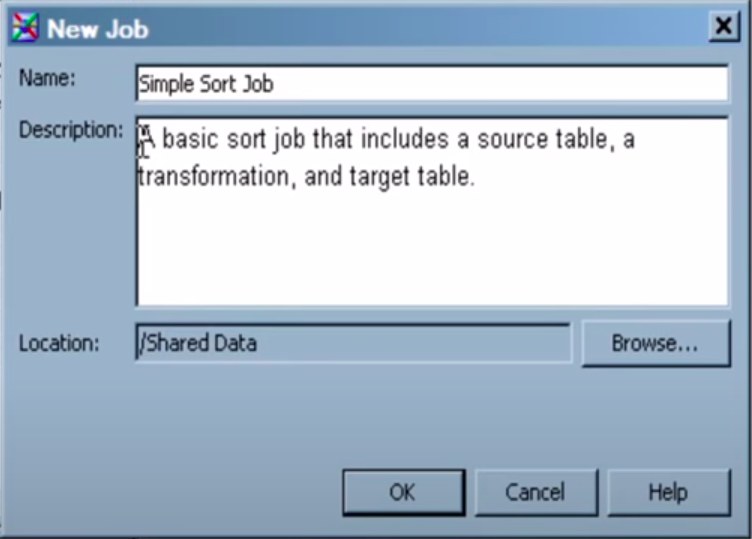
\includegraphics[width=0.85\textwidth]{img/sas_job.png}
		\caption{Демонстрация создания задачи во встроенном редакторе jobs editor программного обеспечения SAS Data Integration Studio}
		\label{analysis:sas_create_job}}
\end{figure}

\newpage

После создания задачи открывается холст на котором возможно располагать графические примитивы, которые впоследствии 
будут преобразованы в запрос. % преобразования над данными.
Некоторые возможные преобразования представлены на рисунке \ref{analysis:sas_job_transform_data}. 
% Все представленные преобразования можно располагать на холсте. 
При расположении на холсте каждое преобразование превращается в графический 
примитив с данными о выполняемом преобразовании.
На рисунке \ref{analysis:sas_simple_job_example} продемонстрирована созданная задача.

\begin{figure}[ht!]
	\centering{
		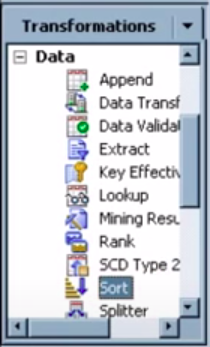
\includegraphics[width=0.4\textwidth]{img/sas_job3.png}
		\caption{Демонстрация панели трансформации во встроенном редакторе jobs editor программного обеспечения SAS Data Integration Studio}
		\label{analysis:sas_job_transform_data}}
\end{figure}

\begin{figure}[ht!]
	\centering{
		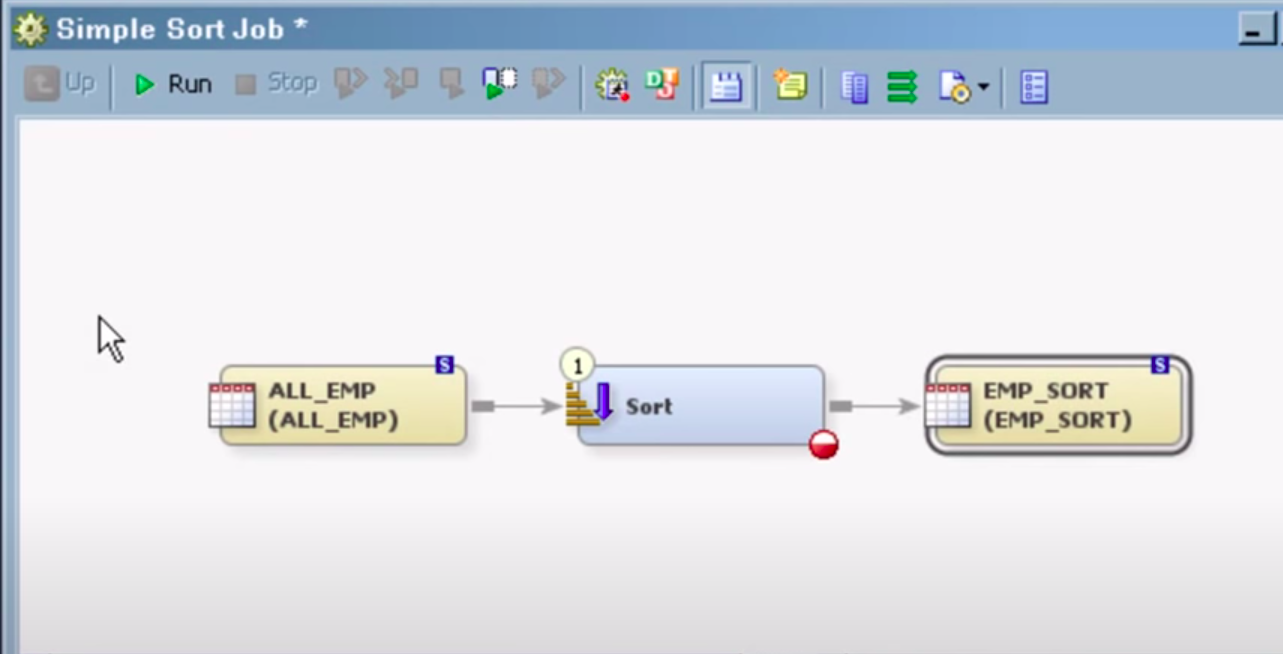
\includegraphics[width=0.75\textwidth]{img/sas_job2.png}
		\caption{Демонстрация созданной задачи во встроенном редакторе jobs editor программного обеспечения SAS Data Integration Studio}
		\label{analysis:sas_simple_job_example}}
\end{figure}

При построении процессов чаще всего применяется сочетание стандартных преобразований 
и написанного пользователем кода (рисунок \ref{analysis:sas2}).
Стандартные преобразования ограничены и могут привести к неэффективной обработке, а иногда и 
к чрезмерно сложным процессам \cite{bib13}. 

\begin{figure}[ht!]
	\centering{
		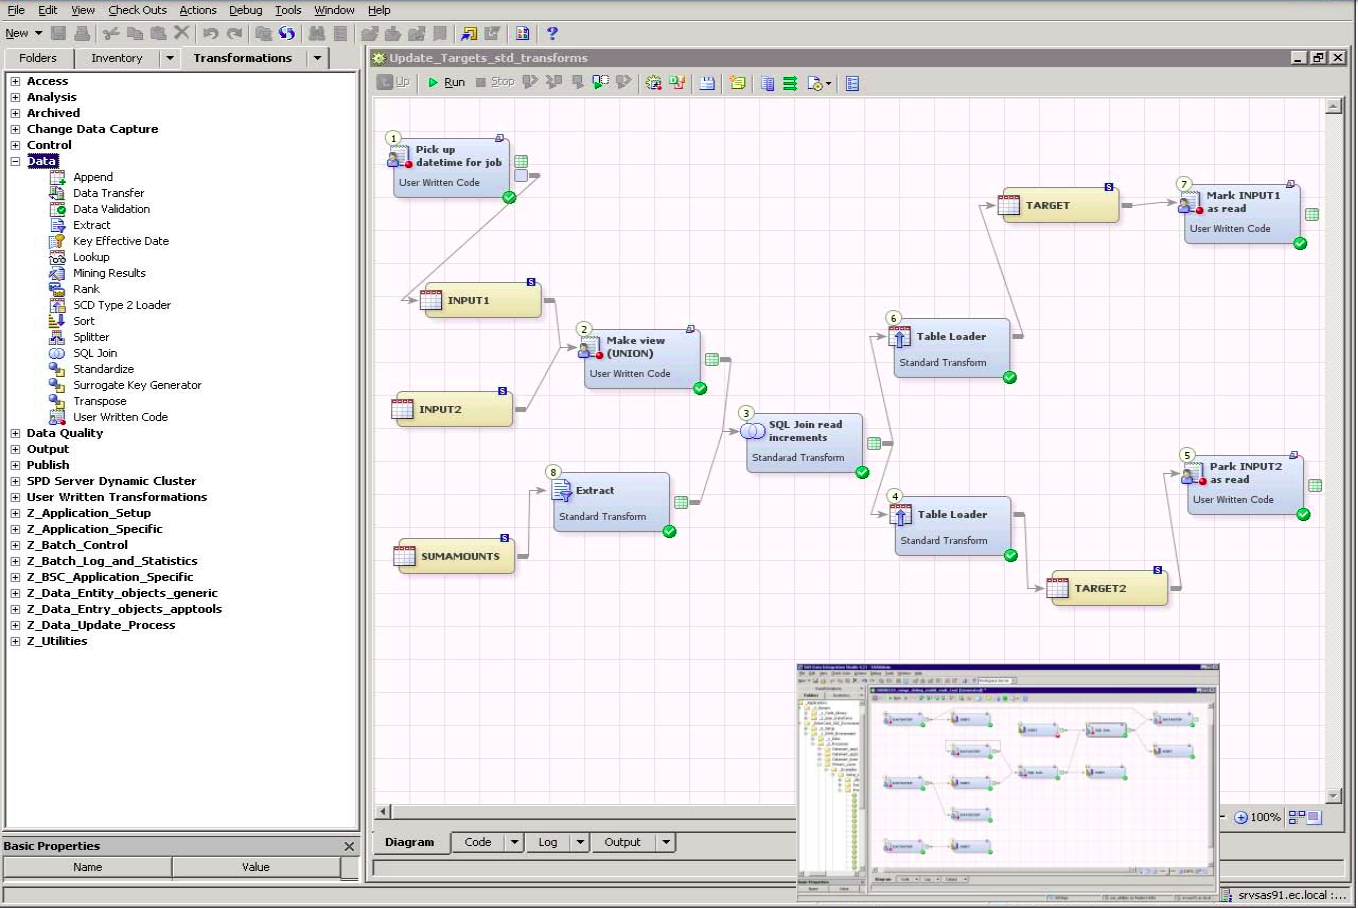
\includegraphics[width=1\textwidth]{img/Sas2.png}
		\caption{Демонстрация собственного кода в SAS Data Integration Studio}
		\label{analysis:sas2}}
\end{figure}

Этапы обработки данных, выполнение соединений, обеспечивает хороший контроль и гибкие
манипуляции с данными, и из-за этого они часто предпочтительнее SQL-соединений.  
Кроме того, полная детализация всех потоков данных не обязательно должна отображаться 
на диаграммах процессов до тех пор, пока не будут охвачены входные и выходные данные постоянных таблиц.
На рисунке \ref{analysis:sas1} представлена работа с тремя источниками данных и двумя выходными таблицами.

\begin{figure}[ht!]
	\centering{
		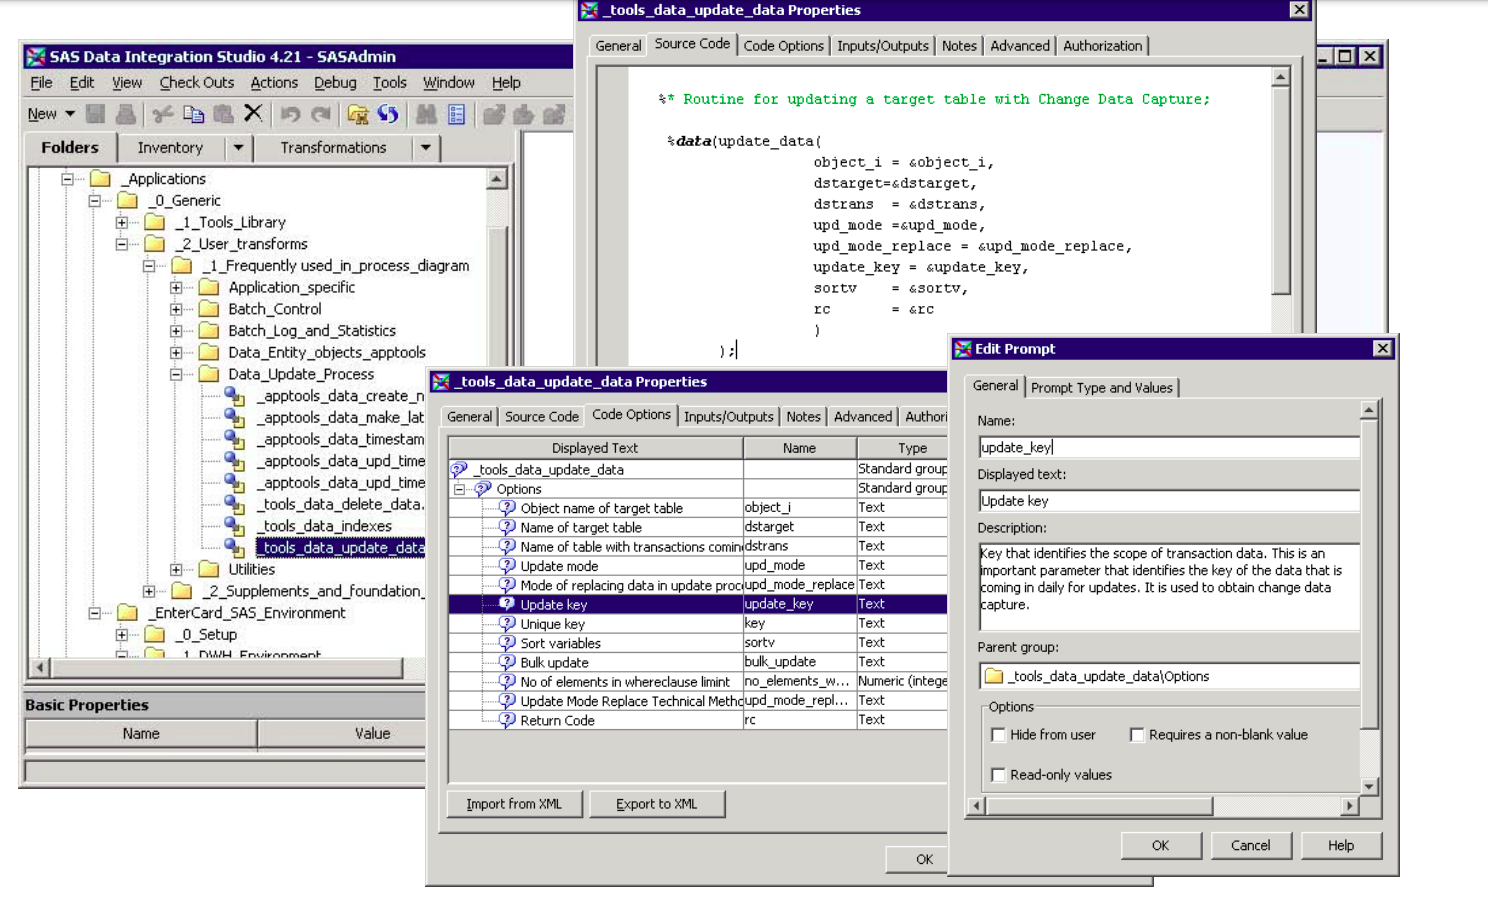
\includegraphics[width=1\textwidth]{img/Sas1.png}
		\caption{Демонстрация работы с тремя источниками данных и двумя выходными таблицами в SAS Data Integration Studio}
		\label{analysis:sas1}}
\end{figure}

На рисунке \ref{analysis:sas3} показано задание проекта в SAS Data Integration Studio, в котором каждый шаг выполняется последовательно \cite{bib14}. 
В этом примере разработчик объединяет пять таблиц с помощью одного ключа, переменной с именем account\_rk. 
Каждая таблица содержит одну и ту же совокупность кредитов, что позволяет выполнять преобразования SQL join в любом порядке. 
Несмотря на отсутствие зависимостей, характер пользовательского интерфейса 
SAS Data Integration Studio позволяет разработчику разрабатывать последовательный процесс. 
Разработчик сначала присоединяется к таблицам Financial\_Account и Counterparty. 
Как только этот шаг будет завершен, результат будет присоединен к таблице адресов. 
Затем результаты объединяются с таблицами Risk\_Rating и Account\_Status. 
Из-за последовательной конструкции четыре преобразования SQL Join выполняются по одному за раз.

\begin{figure}[ht!]
	\centering{
		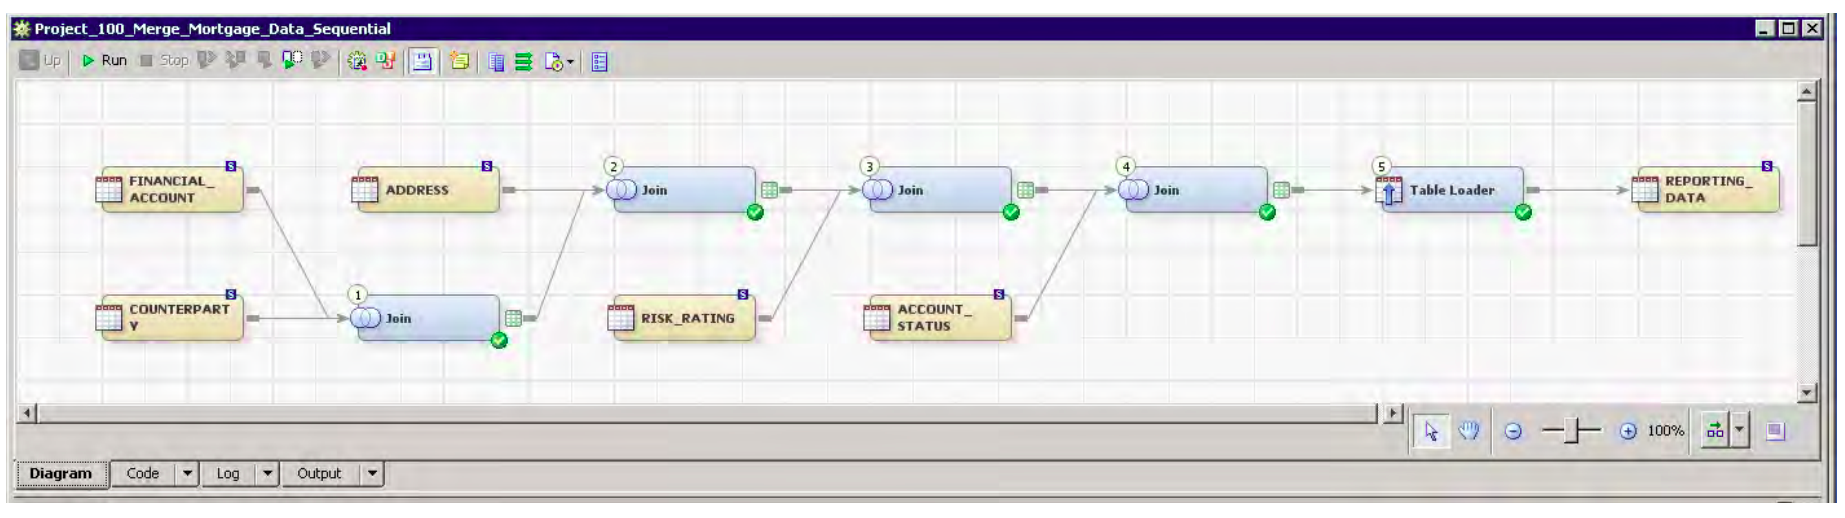
\includegraphics[width=1\textwidth]{img/Sas3.png}
		\caption{Демонстрация работы SAS Data Integration Studio с последовательными шагами}
		\label{analysis:sas3}}
\end{figure}

\newpage

\subsection{Informatica PowerCenter}

\textit{Informatica PowerCenter} -- платформа интеграции данных, основанная на 
работе со структурами данных в визуальной среде \cite{bib3}.  
Данная платформа предоставляет возможность работать со структурами данных 
без написания программного кода, что позваоляет не только ускорить получение данных бизнесом,
но и облегчить взаимодействие с данными пользователям. 

Пользовательский интерфейс инструмента разработчика состоит из рабочей среды с несколькими представлениями,
которые используются для создания решений, для интеграции данных и объединения данных.
На рисунке \ref{analysis:informatica_interface} показан пользовательский интерфейс. 
В него входят следующие инструменты.

\begin{enumerate}
   \item Просмотр обозревателя объектов.
   \item Общий вид.
   \item Просмотр свойств.
   \item Просмотр данных.
   \item Просмотр тегов.
   \item Представление зависимостей объектов.
   \item Просмотр оповещений.
   \item Просмотр проводника подключений.
   \item Редактор.
\end{enumerate}

\begin{figure}[ht!]
	\centering{
		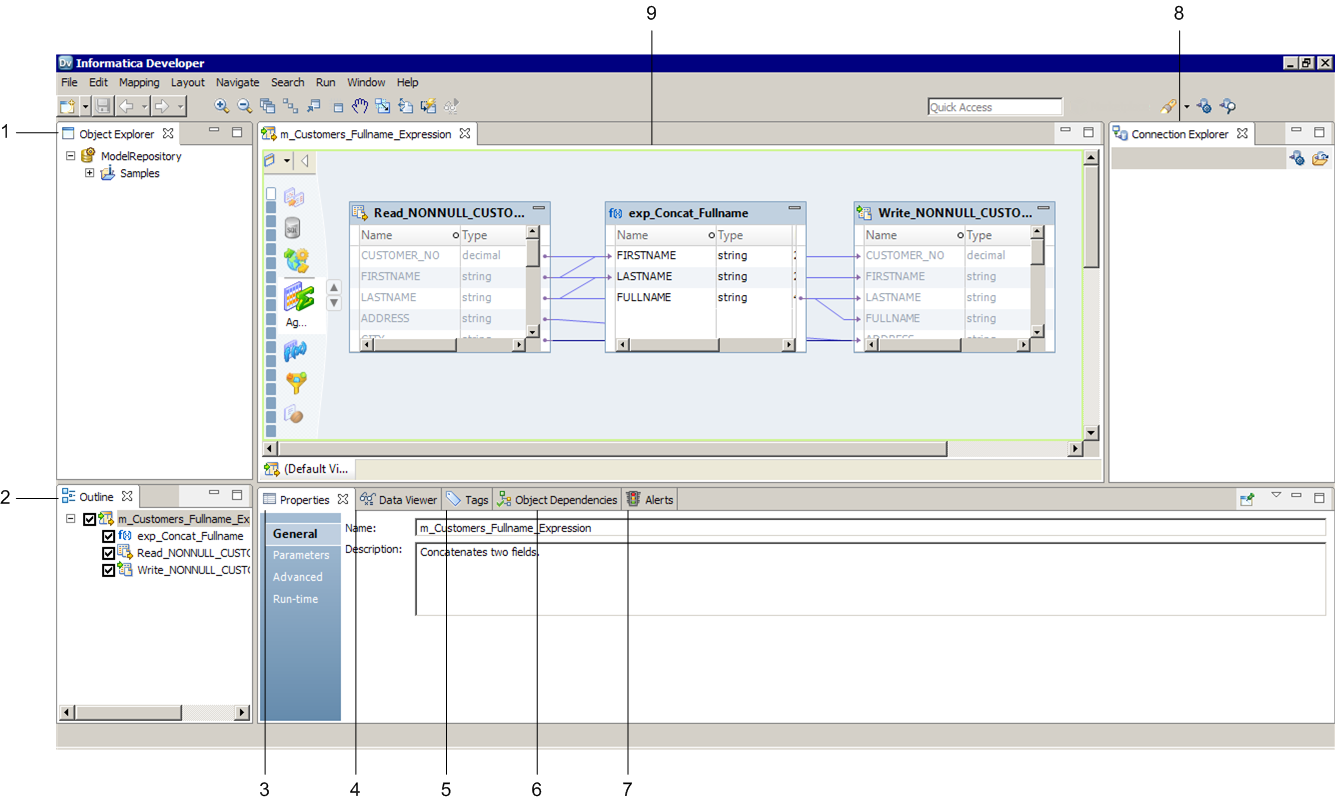
\includegraphics[width=1\textwidth]{img/informatica3.png}
		\caption{Пользовательский интерфейс в платформе Informatica PowerCenter}
		\label{analysis:informatica_interface}}
\end{figure}

Инструмент разработчика может отображать следующие представления.
\begin{enumerate}
   \item Просмотр обозревателя объектов - отображает проекты, папки и объекты внутри проектов и папок.
   \item Просмотр проводника подключений - отображает подключения к реляционным базам данных.
   \item Общий вид - отображает объекты, зависящие от объекта, выбранного в представлении обозревателя объектов.
   \item Просмотр шпаргалок -  отображает открытую шпаргалку.
   \item Просмотр данных - отображает исходные данные, результаты профиля и предварительный просмотр результатов преобразования. 
   \item Представление зависимостей объектов - отображает зависимости объектов при просмотре, изменении или удалении объекта.
   \item Просмотр оповещений - отображает предупреждения о состоянии соединения.
   \item Просмотр журнала проверки - отображает ошибки проверки объекта.
\end{enumerate}

На рисунке \ref{analysis:informatica_edit_transf} показано окно изменения данных. 
На рисунке \ref{analysis:informatica_canvas} показан холст, на котором расположены графические 
элементы, связанные между собой. 

\begin{figure}[ht!]
	\centering{
		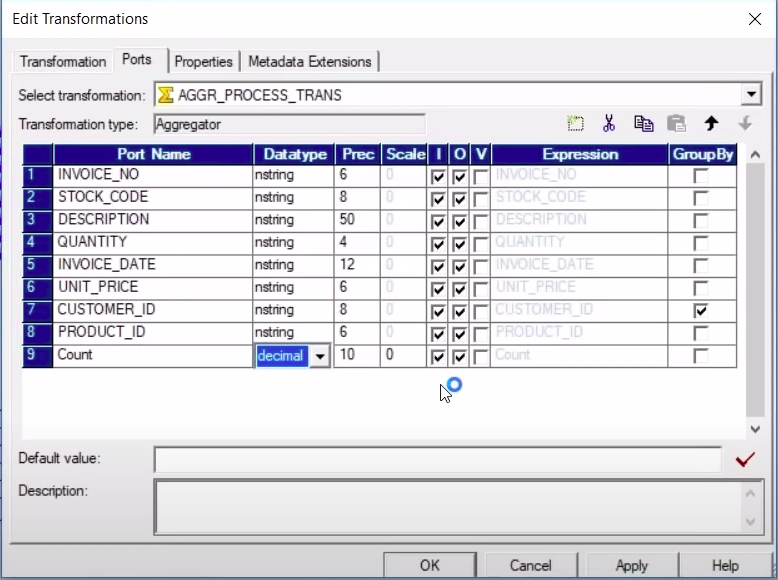
\includegraphics[width=0.95\textwidth]{img/informatica1.png}
		\caption{Окно изменения данных в платформе Informatica PowerCenter}
		\label{analysis:informatica_edit_transf}}
\end{figure}

\begin{figure}[ht!]
	\centering{
		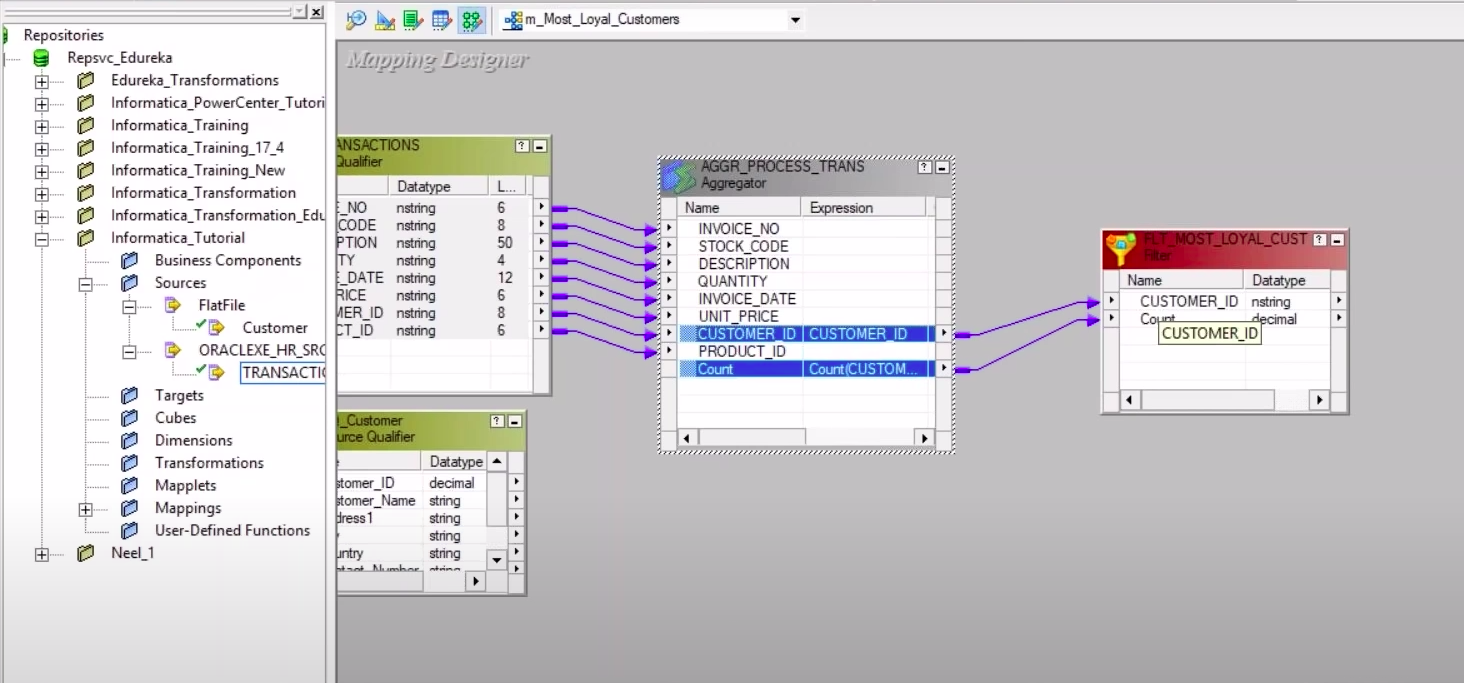
\includegraphics[width=0.95\textwidth]{img/informatica2.png}
		\caption{Холст в платформе Informatica PowerCenter}
		\label{analysis:informatica_canvas}}
\end{figure}

На рисунке \ref{analysis:informatica3} показан пример преобразования данных при помощи пассивной трансформации \cite{bib15}. 
Пассивное преобразование не изменяет количество строк, проходящих через преобразование, сохраняет границу транзакции и сохраняет тип строки.
Преобразование может быть подключено к потоку данных с помощью портов ввода/вывода к любому другому преобразованию или источнику/цели.
Порты преобразования разделяются на  входные, входные/выходные, переменные и выходные порты. Порты ввода/вывода принимает данные и передает их без изменений.
Также поддерживаются многогрупповые преобразования, являющиеся преобразованиями 
имеющее несколько входных и выходных групп.

\begin{figure}[ht!]
	\centering{
		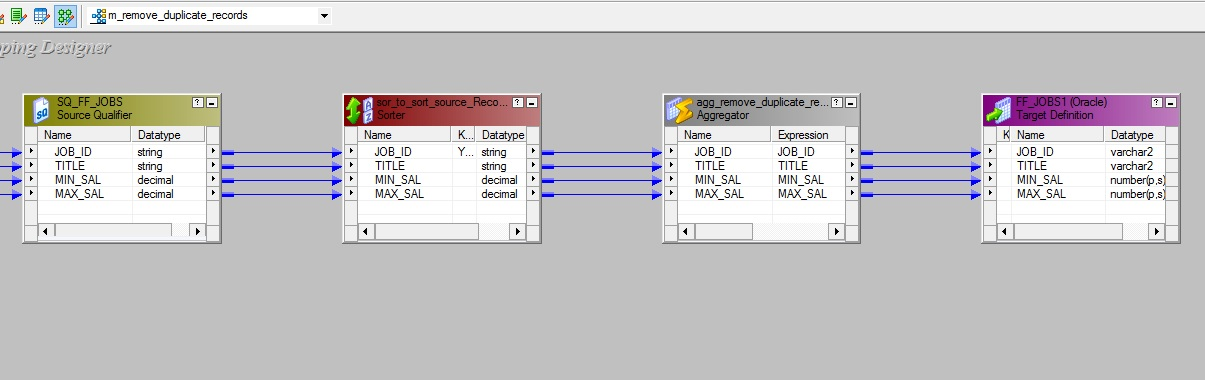
\includegraphics[width=1\textwidth]{img/informatica3.jpg}
		\caption{Пример преобразования данных в платформе Informatica PowerCenter}
		\label{analysis:informatica3}}
\end{figure}

\newpage

\subsection{Apache NiFi}

\textit{Apache NiFi} -- это программный проект от Apache Software Foundation, предназначенный для обработки информации, 
предоставляющий возможности управления потоками 
данных из разнообразных источников в режиме реального времени с использованием графического интерфейса \cite{bib4}. 
В NiFi используется веб-интерфейс для создания потоков данных.

Пользовательский интерфейс NiFi предоставляет механизмы для
создания автоматизированных потоков данных, а также визуализации, редактирования, мониторинга и администрирования этих потоков данных.
Пользовательский интерфейс можно разбить на несколько сегментов, каждый из которых отвечает за различные функции приложения.

Когда приложение запускается, пользователь может перейти к пользовательскому интерфейсу, 
перейдя по адресу по умолчанию https://localhost:8443/nifi в веб-браузере. 
Конфигурация по умолчанию создает имя пользователя и пароль с полными правами администратора системы. 
NiFi также предоставляет возможность защиты системы.

На рисунке \ref{analysis:nifi1} представлен пустой холст, на котором можно построить поток данных:

\begin{figure}[ht!]
	\centering{
		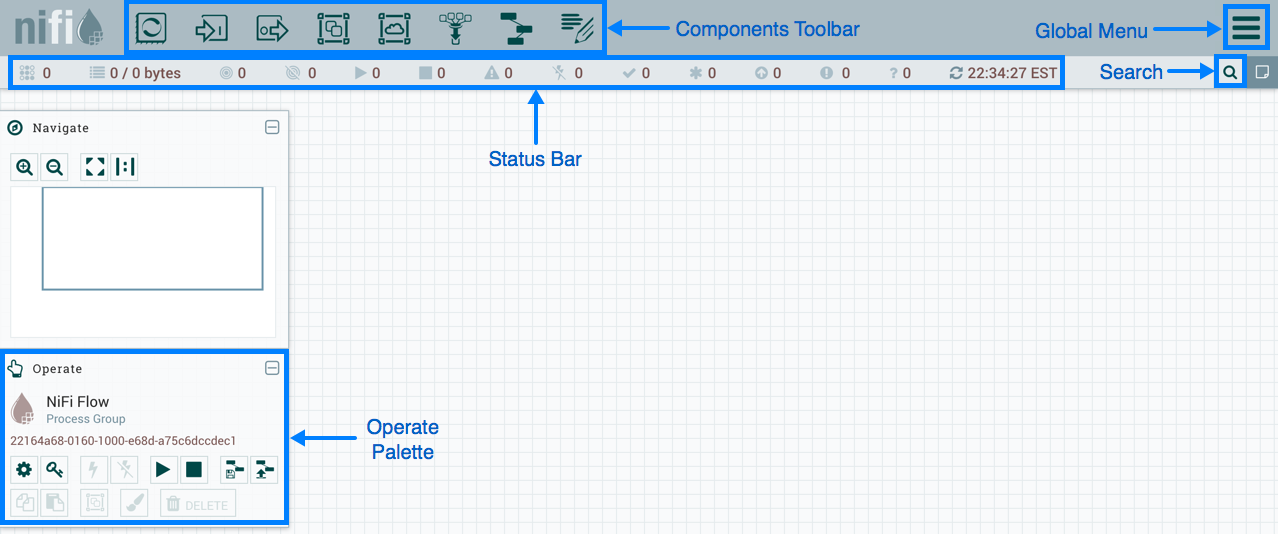
\includegraphics[width=1\textwidth]{img/nifi1.png}
		\caption{Пример пустого холста в программном продукте Apache NiFi}
		\label{analysis:nifi1}}
\end{figure}

Панель инструментов компонентов располагается в верхней левой части экрана. 
Она состоит из компонентов, которые можно перетаскивать на холст, чтобы создать поток данных. 
После того, как пользователь перетаскивает компонент на холст, он может взаимодействовать с ним, щелкнув 
по компоненту правой кнопкой мыши и выбрав параметр в контекстном меню рисунок \ref{analysis:nifi2}. 
Параметры, доступные пользователю в контекстном меню, различаются в зависимости от назначенных ему привилегий.

\begin{figure}[ht!]
	\centering{
		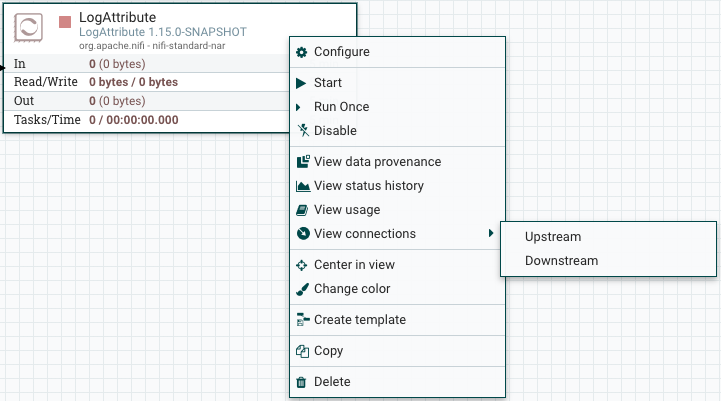
\includegraphics[width=1\textwidth]{img/nifi2.png}
		\caption{Пример контекстного меню для компонента в программном продукте Apache NiFi}
		\label{analysis:nifi2}}
\end{figure}

На рис. \ref{analysis:nifi_example} и рис. \ref{analysis:nifi_example2}  показаны холсты, на которых созданы потоки данных.
NiFi позволяет парсить данные регулярными выражениями, выполнять по ним sql, 
фильтровать и добавлять поля, конвертировать один формат данных в другой \cite{bib11}. 

\begin{figure}[ht!]
	\centering{
		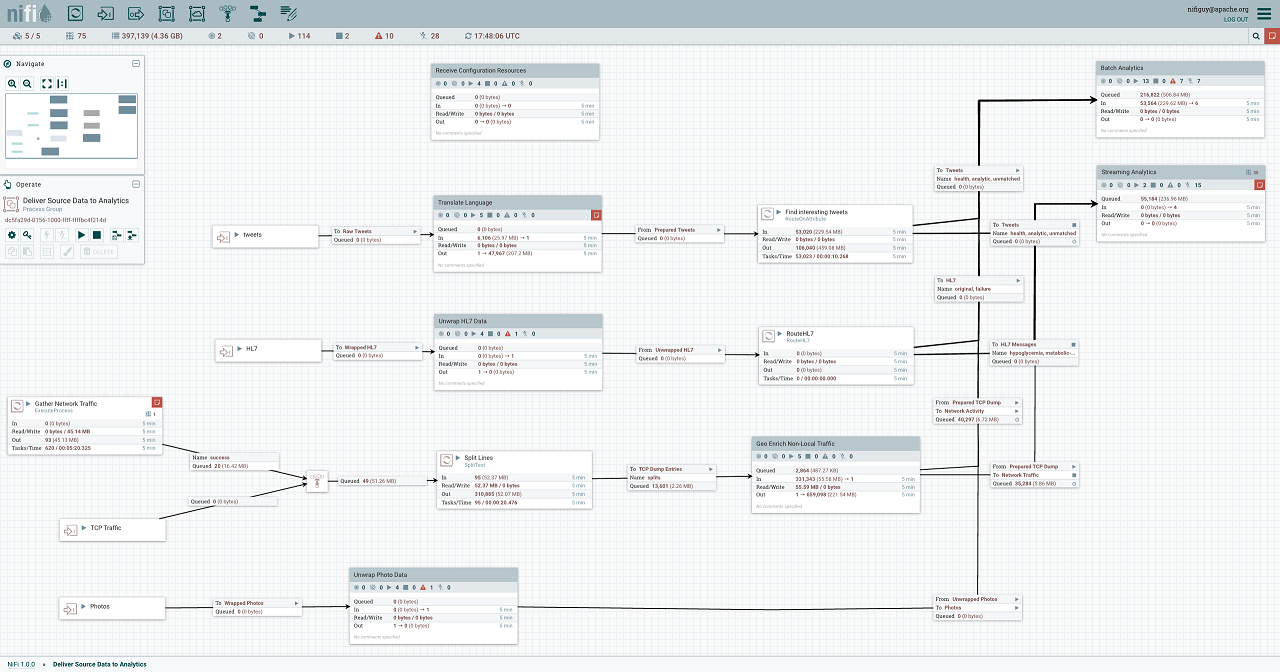
\includegraphics[width=1\textwidth]{img/nifi_example.png}
		\caption{Пример потока данных в программном продукте Apache NiFi}
		\label{analysis:nifi_example}}
\end{figure}

\begin{figure}[ht!]
	\centering{
		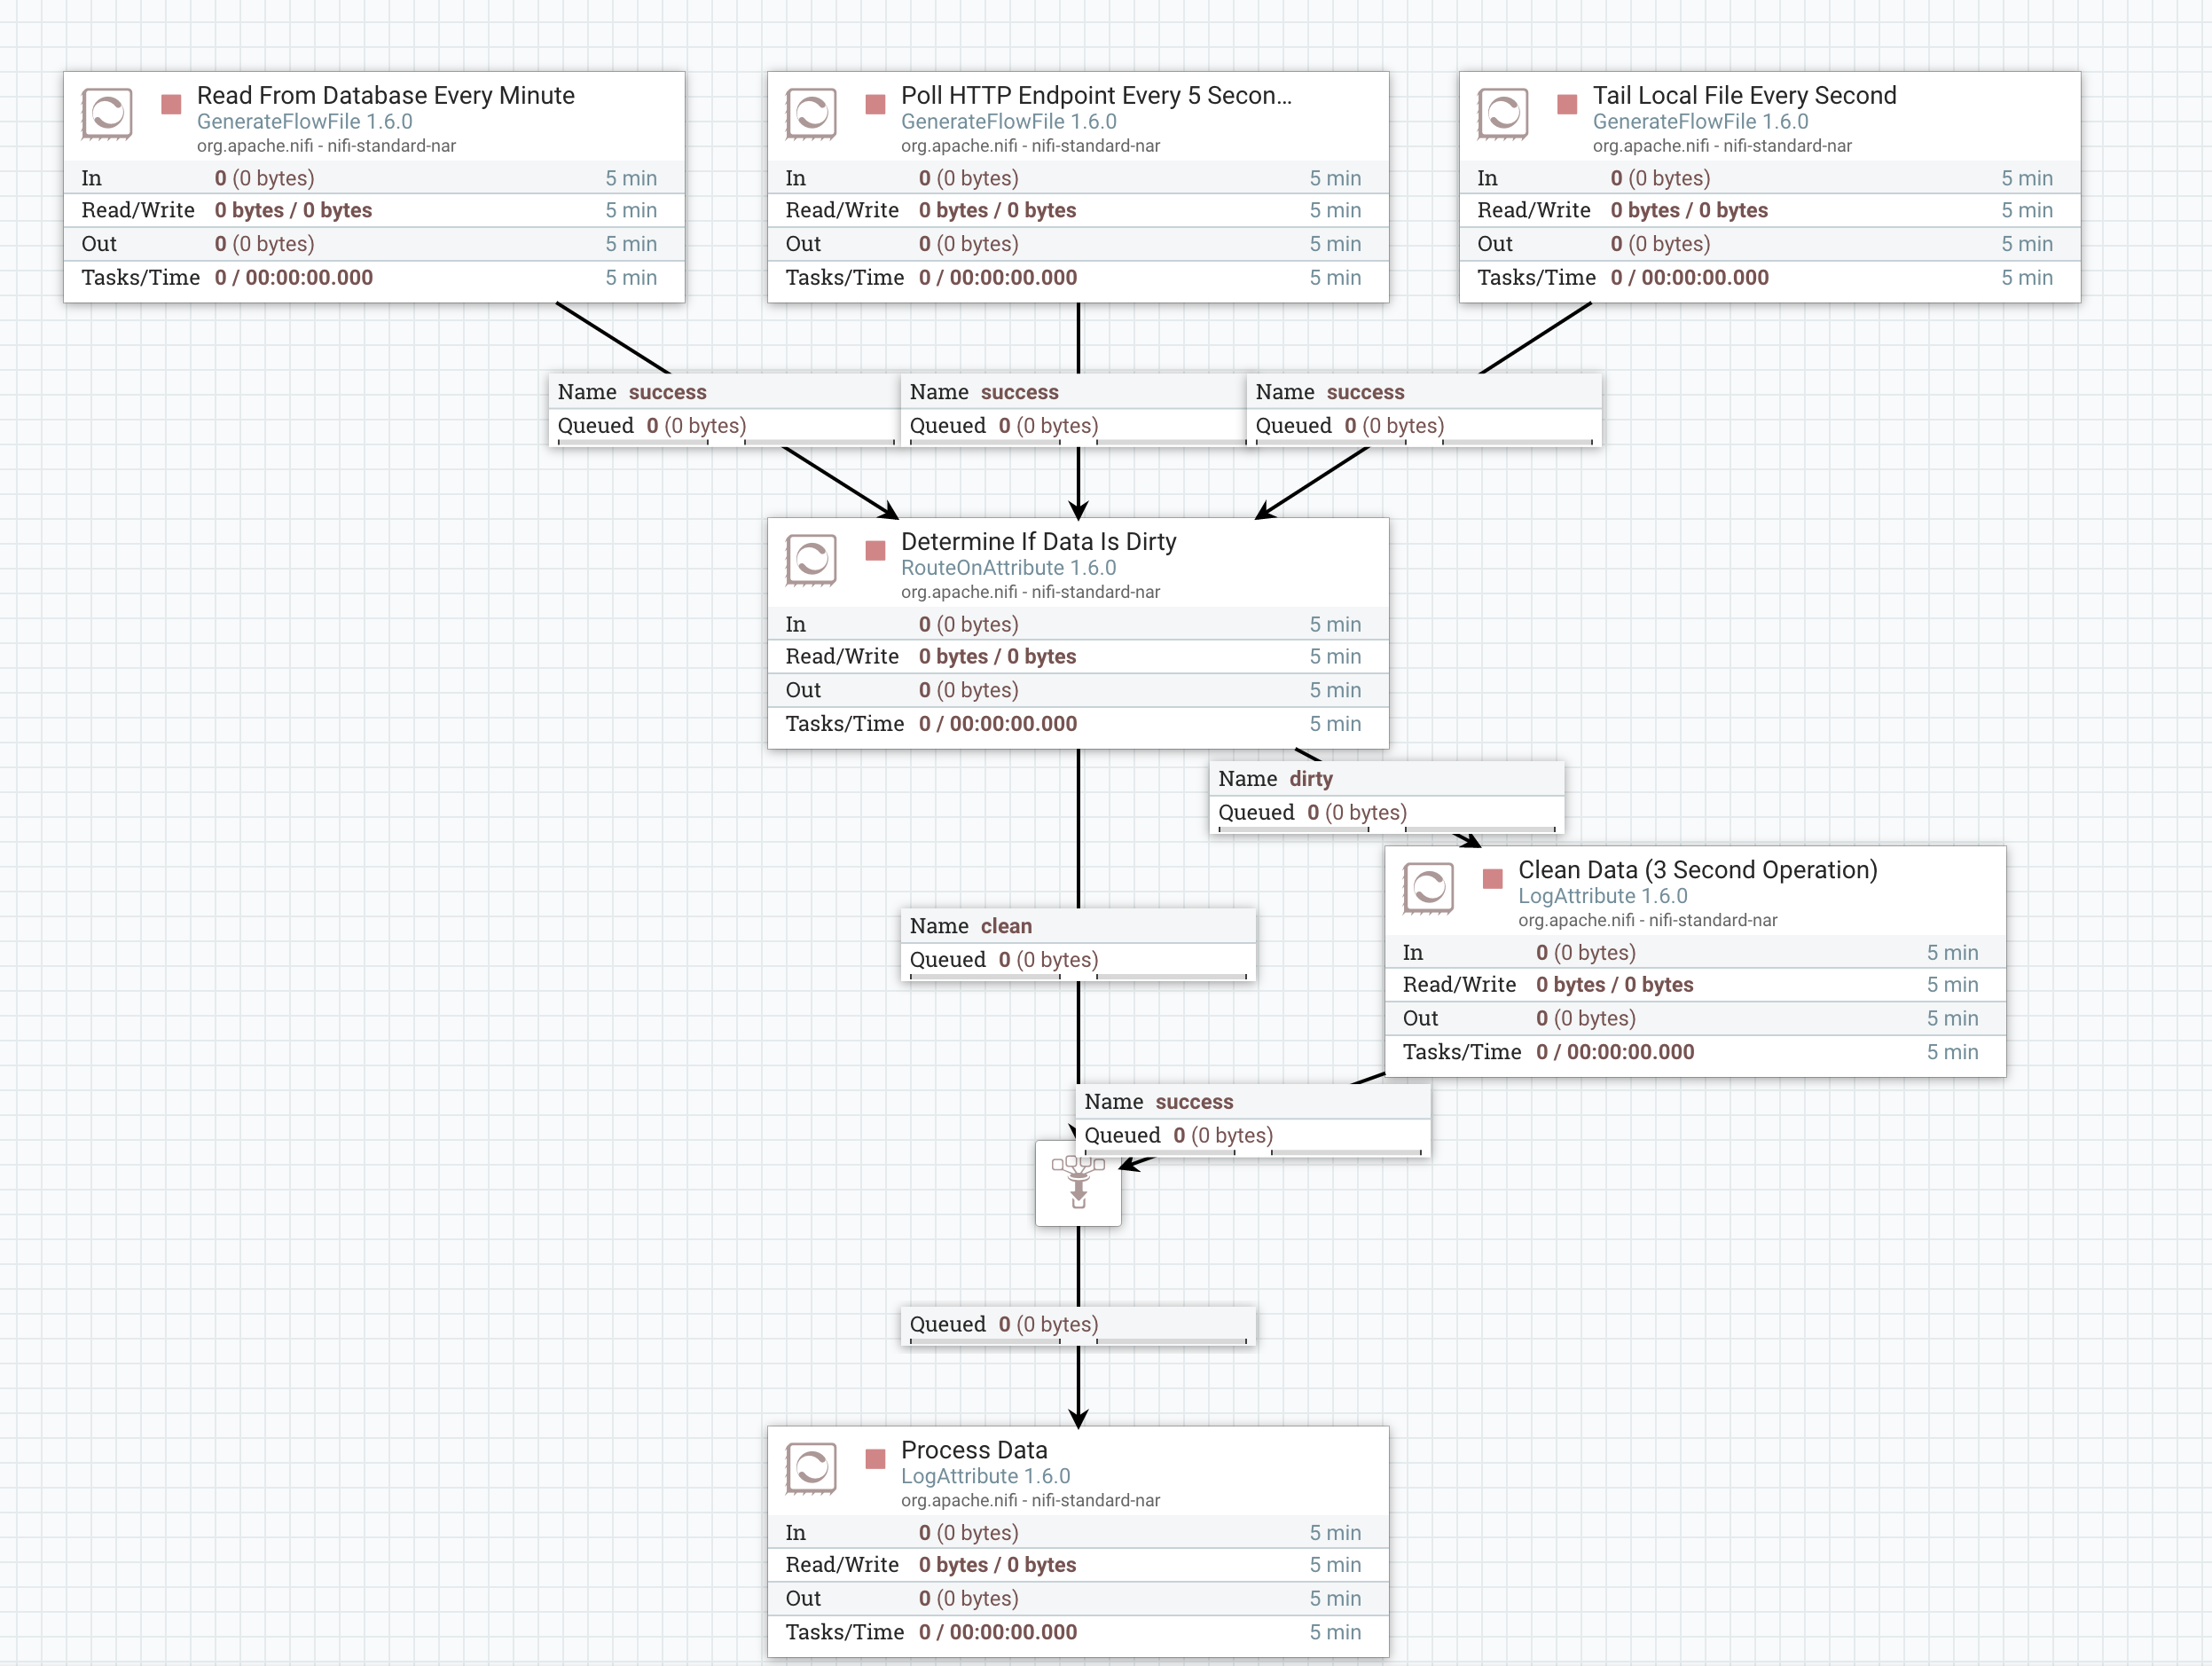
\includegraphics[width=1\textwidth]{img/nifi_example2.png}
		\caption{Второй пример потока данных в программном продукте Apache NiFi}
		\label{analysis:nifi_example2}}
\end{figure}

\newpage

\subsection{DBForge Studio}

DBForge Studio \cite{bib16} - это графический инструмент для разработки, управления и администрирования баз данных. 
Данный продукт позволяет создавать и выполнять запросы, разрабатывать и отлаживать хранимые процедуры, автоматизировать управление объектами базы данных,
анализировать табличные данные с помощью интерфейса. 

DB Forge Studio позволяет оформлять таблицы в визуальном редакторе \ref{analysis:dbForge1}.
Конструктор таблиц содержит визуальные редакторы для столбцов, индексов,
первичных и внешних ключей, проверочных ограничений, 
статистики и свойств хранения таблицы. 
Он позволяет редактировать данные таблицы, 
синхронно перемещаться по визуальному редактору и редактору T-SQL, использовать 
автоматические подсказки типов данных, документировать таблицы, 
предварительно просматривать сценарии ALTER TABLE и перестраивать таблицу без потери ее данных.


\begin{figure}[ht!]
	\centering{
		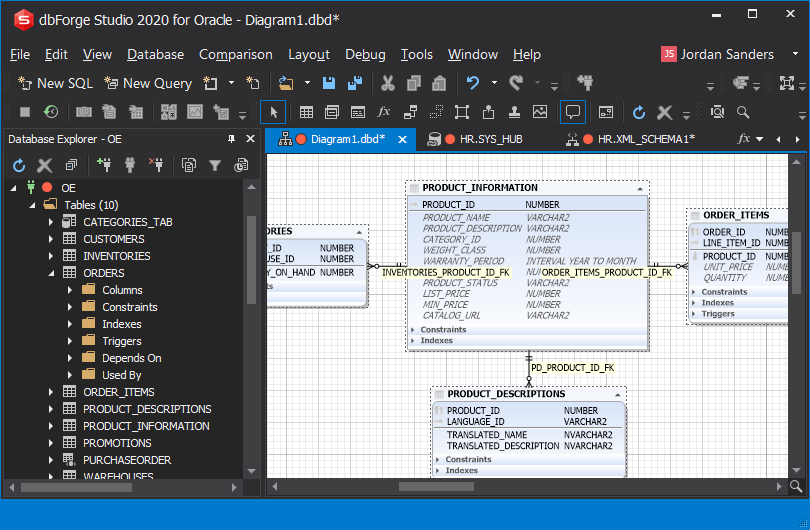
\includegraphics[width=1\textwidth]{img/dbForge1.png}
		\caption{Визуальном редактор программного продукта DBForge Studio}
		\label{analysis:dbForge1}}
\end{figure}   
 
\begin{figure}[ht!]
   \centering{
      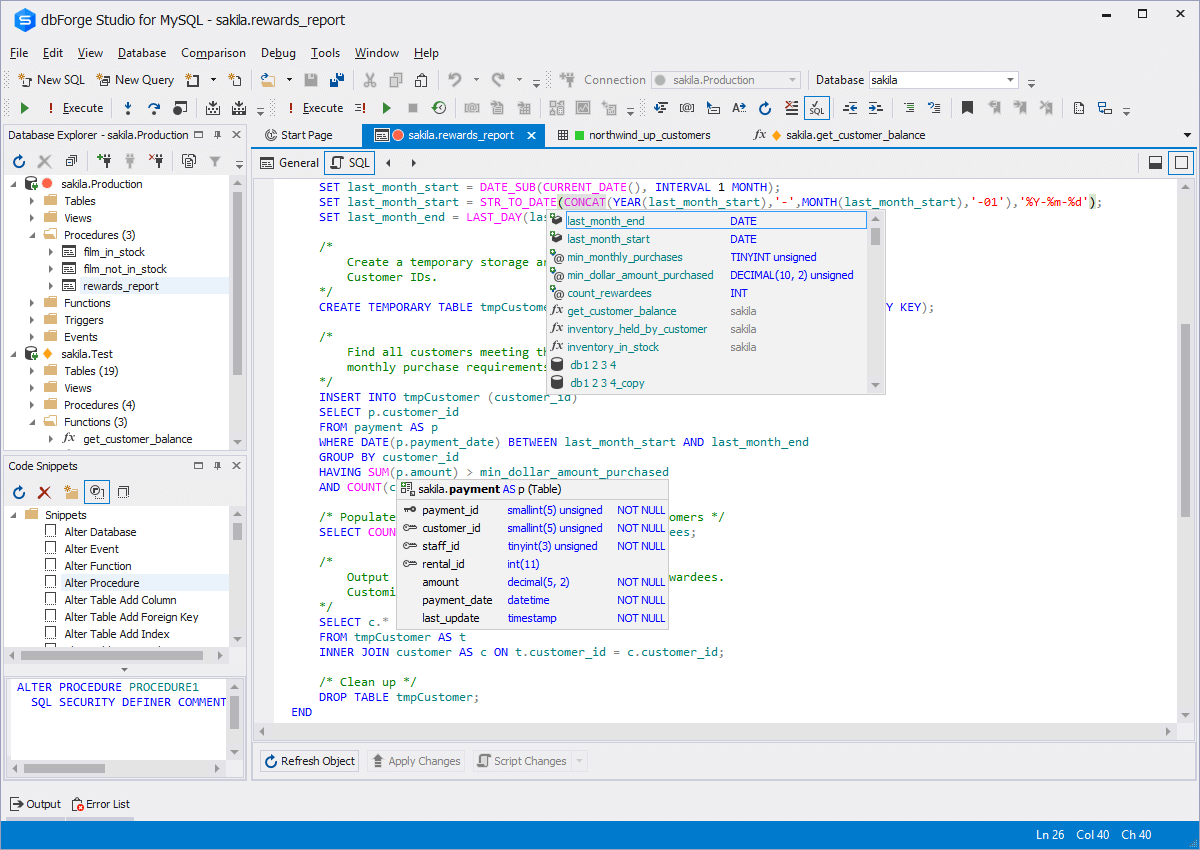
\includegraphics[width=1\textwidth]{img/dbForge2.png}
      \caption{Возможность написания собственного кода в программном продукте DBForge Studio}
      \label{analysis:dbForge2}}
\end{figure}

\begin{figure}[ht!]
	\centering{
		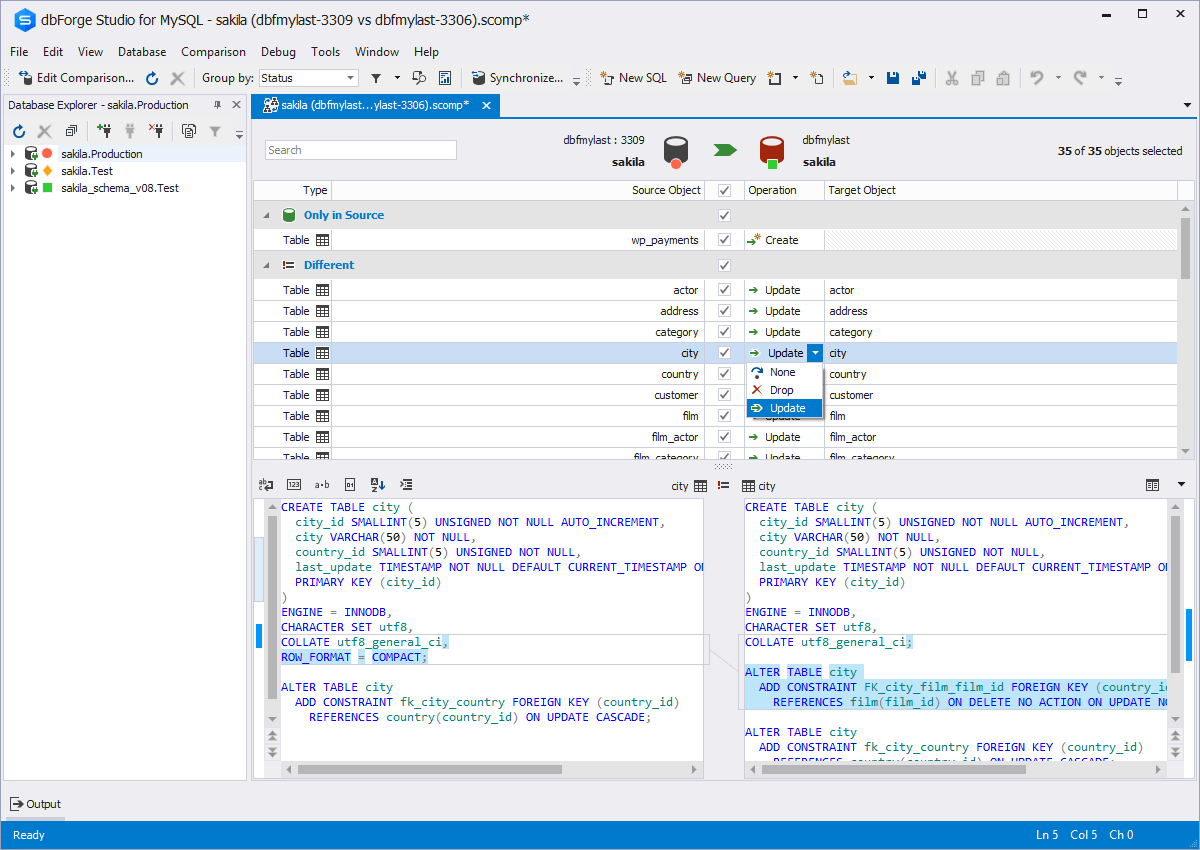
\includegraphics[width=1\textwidth]{img/dbForge3.png}
		\caption{Возможность сравнения и синхронизации баз данных в программном продукте DBForge Studio}
		\label{analysis:dbForge3}}
\end{figure}

\begin{figure}[ht!]
	\centering{
		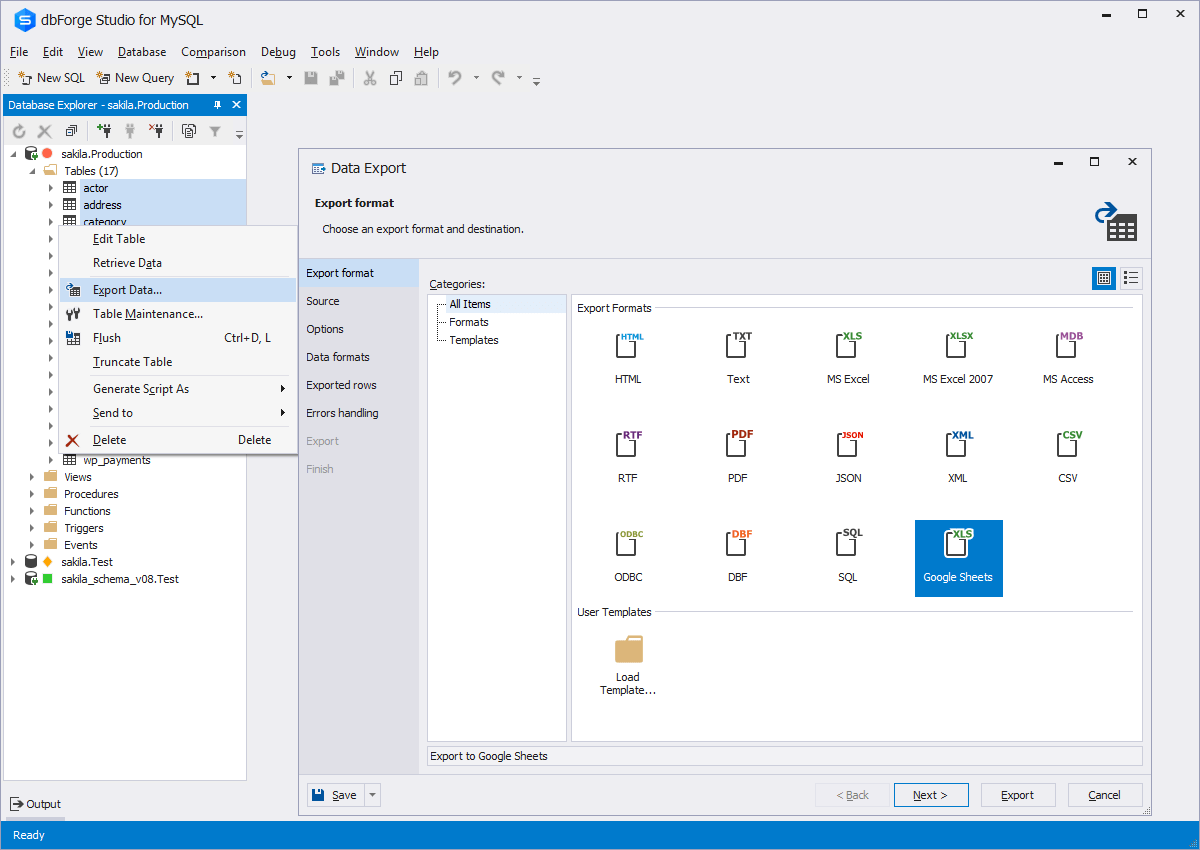
\includegraphics[width=1\textwidth]{img/dbForge4.png}
		\caption{Импорт/экспорт данных в программном продукте DBForge Studio}
		\label{analysis:dbForge4}}
\end{figure}   


DB Forge Studio позволяет рисовать структуры базы данных на диаграммах сущность-связь,
создавать схему базы данных, чтобы визуализировать ее структуру и логические связи между таблицами,
редактировать объекты базы данных прямо на диаграмме, 
кластеризовать логически связанные объекты с помощью контейнеров. 
печатать большие диаграммы базы данных.


Также DBForge Studio поддерживает следующие возможности \cite{bib17}.
\begin{enumerate}
   \item Возможность написания собственного кода с автозавершением кода (рис \ref{analysis:dbForge2}).   
   \item Сравнение и синхронизация баз данных (рис \ref{analysis:dbForge3}) при изменении структуры базы данных, переносе данных между серверами, анализе различий между базами данных.
   \item Импорт/экспорт данных (рис \ref{analysis:dbForge4}). Заполните базы данных MySQL внешними данными. Поддерживается более 10 форматов данных. Позволяет настраивать весь процесс импорта/экспорта.
   \item Копирование баз данных (рис \ref{analysis:dbForge5}).
   \item Дизайнер баз данных (рис \ref{analysis:dbForge6}). Используется  для создания, анализа, обратного проектирования, печати и настройки ваших баз данных, а также  просмотра отношений между таблицами, 
   отображение объектов БД со свойствами, выполнение сохраненных подпрограмм.
   \item Визуальный конструктор запросов (рис. \ref{analysis:dbForge7}). 
   Визуальное создание запросов с помощью редактора диаграмм и выражений. 
   Можно создавать запросы любой сложности. 
   Инструмент с графическим интерфейсом автоматически добавляет соединения между таблицами и позволяет работать с операторами INSERT, UPDATE, DELETE.   
\end{enumerate}


\begin{figure}[ht!]
	\centering{
		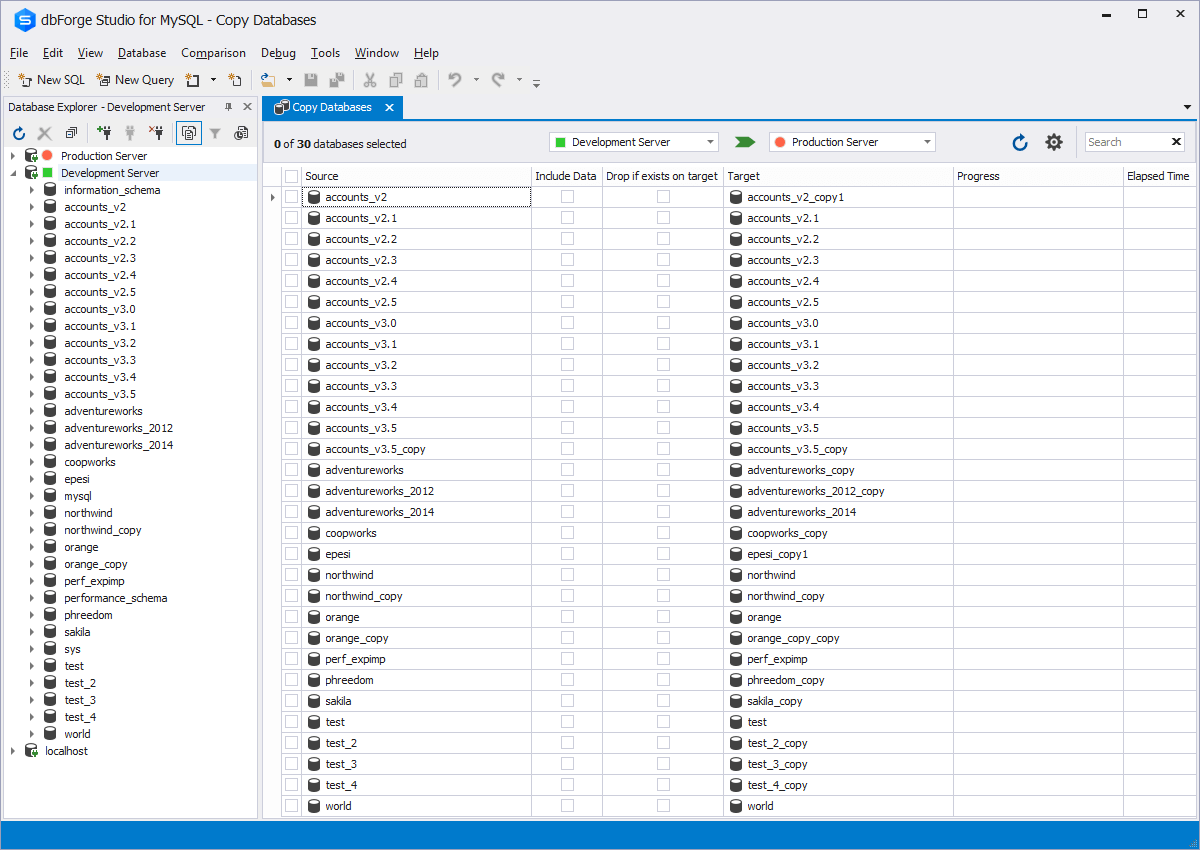
\includegraphics[width=1\textwidth]{img/dbForge5.png}
		\caption{Копирование баз данных в программном продукте DBForge Studio}
		\label{analysis:dbForge5}}
\end{figure}   

\newpage

\begin{figure}[ht!]
	\centering{
		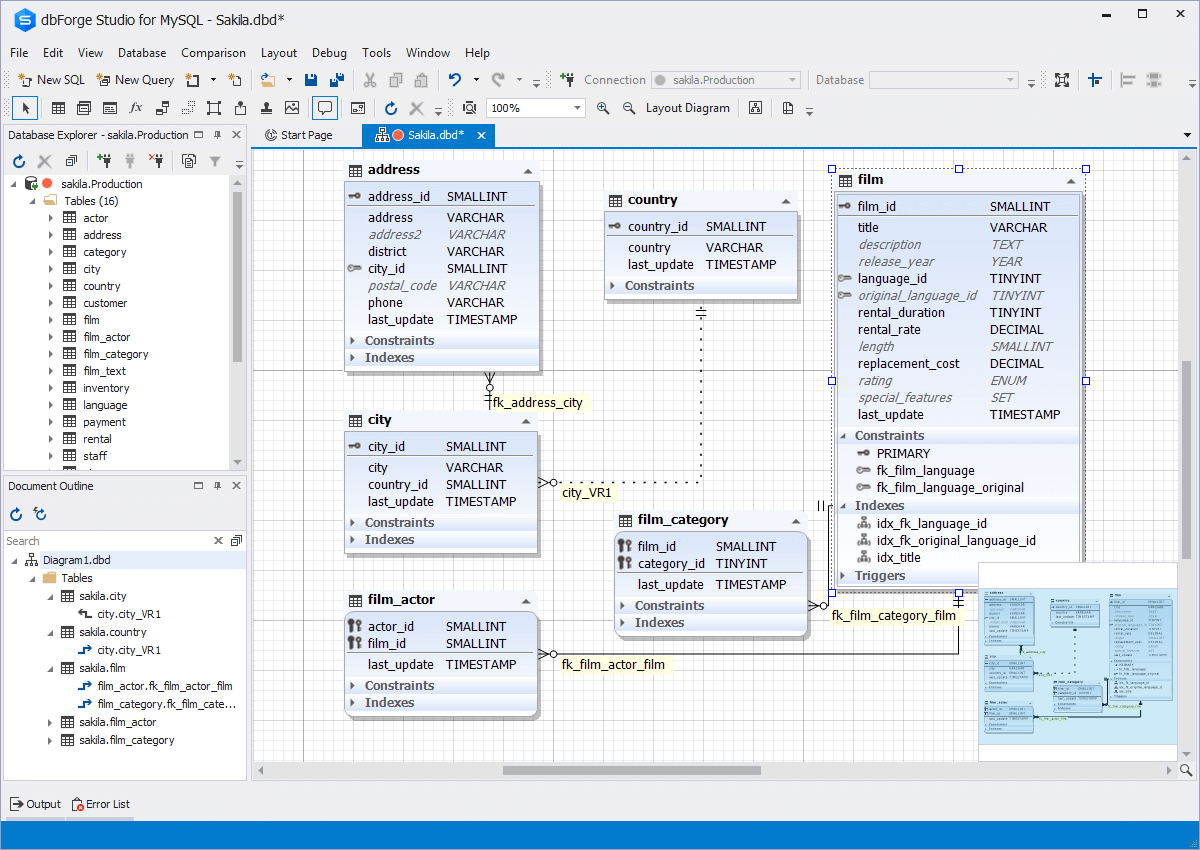
\includegraphics[width=1\textwidth]{img/dbForge6.png}
		\caption{Дизайнер баз данных программного продукта DBForge Studio}
		\label{analysis:dbForge6}}
\end{figure}   

\newpage

\begin{figure}[ht!]
	\centering{
		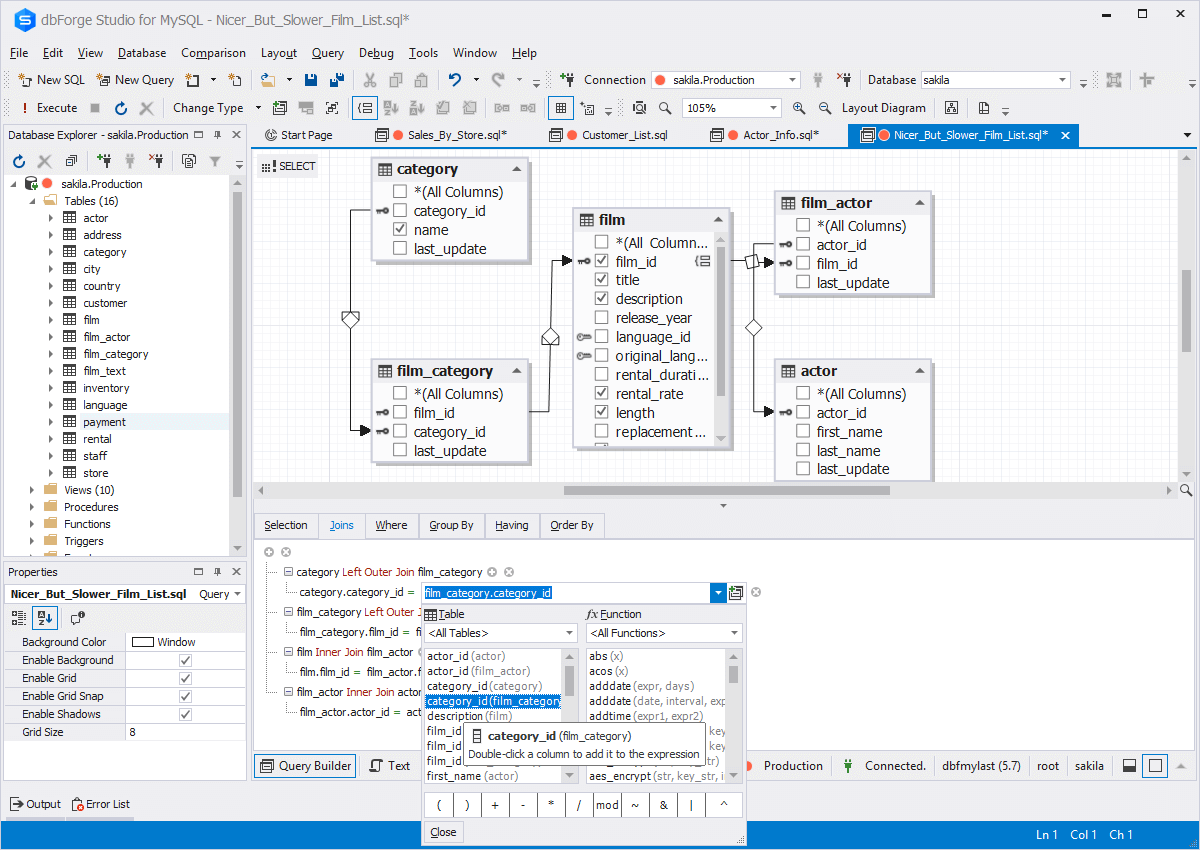
\includegraphics[width=1\textwidth]{img/dbForge7.png}
		\caption{Визуальный конструктор запросов программного продукта DBForge Studio}
		\label{analysis:dbForge7}}
\end{figure}   

Для составления условий предназначена вкладка 'Where' рисунок \ref{analysis:dbForge_1}. 
Также представлены вкладки 'Selection', 'Joins', 'Group By', 'Having' и 'Order by'.

\begin{figure}[ht!]
	\centering{
		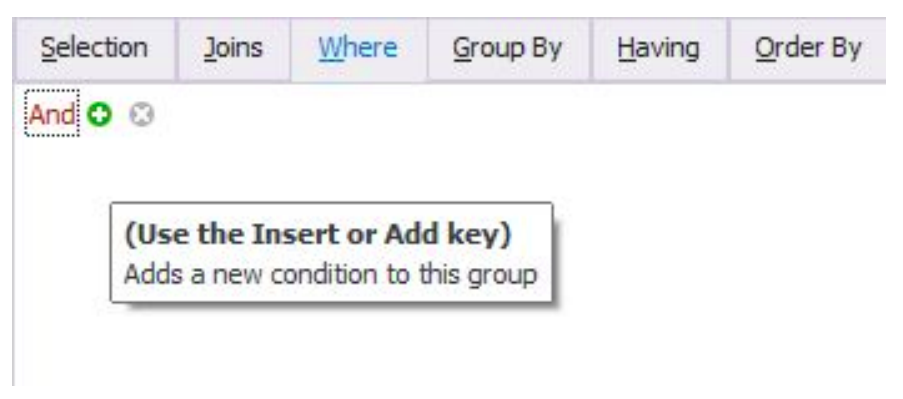
\includegraphics[width=1\textwidth]{img/dbForge_1.png}
		\caption{Выбор условия во вкладка "Where" продукта DBForge Studio}
		\label{analysis:dbForge_1}}
\end{figure}   

\newpage

При составлении условия редактор предлагает выбирать следующие элементы рисунок \ref{analysis:dbForge_2}.

\begin{figure}[ht!]
	\centering{
		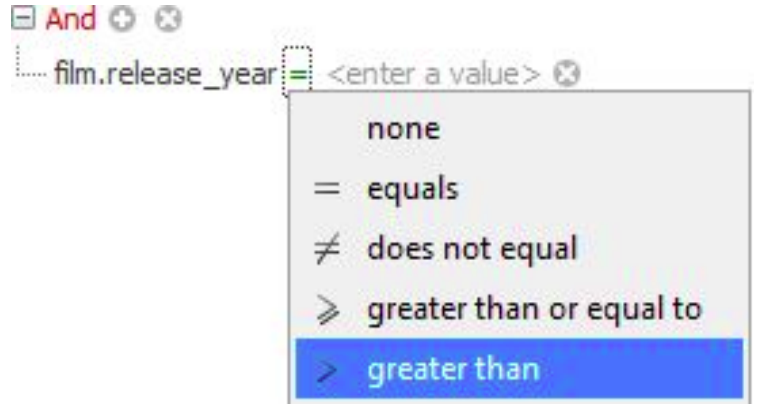
\includegraphics[width=1\textwidth]{img/dbForge_3.png}
		\caption{Выбор условия во вкладка "Where" продукта DBForge Studio}
		\label{analysis:dbForge_2}}
\end{figure}   

\newpage

После составления запроса его можно выполнить и получить результат рисунок \ref{analysis:dbForge_3}.

\begin{figure}[ht!]
	\centering{
		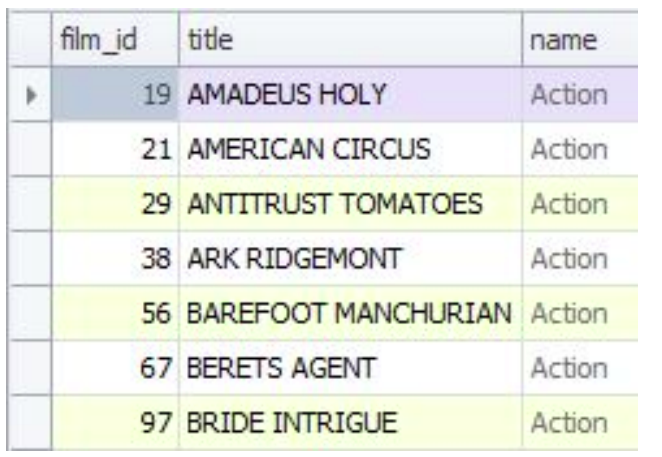
\includegraphics[width=1\textwidth]{img/dbForge_4.png}
		\caption{Результат запроса в продукте DBForge Studio}
		\label{analysis:dbForge_3}}
\end{figure}   

\newpage

После визуализации запроса его можно увидеть в виде строки во вкладке 'SQL' рисунок \ref{analysis:dbForge_5}. 
Во вкладке 'Data' будет представлено выполнение запроса.

\begin{figure}[ht!]
	\centering{
		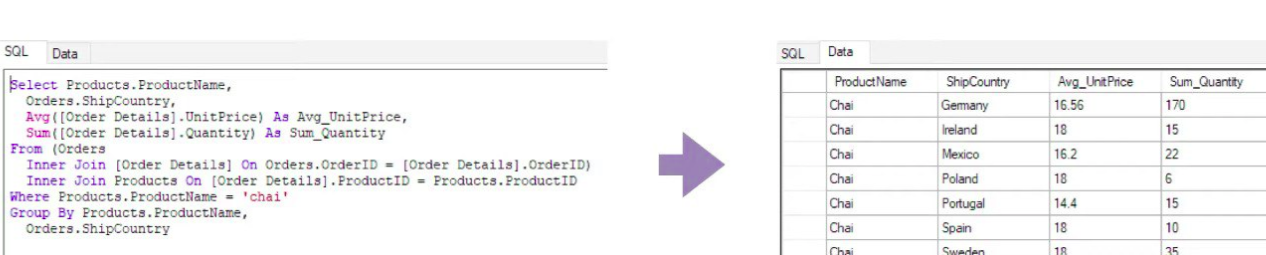
\includegraphics[width=1\textwidth]{img/dbForge_5.png}
		\caption{Представление визуализирумого запроса в виде строки в DBForge Studio}
		\label{analysis:dbForge_5}}
\end{figure}  

\newpage

\subsection{FlySpeed SQL Query}

FlySpeed SQL Query \cite{bib18} - инструмент для работы с базами данных и SQL запросами. 
FlySpeed SQL Query также позволяет работать с офисными форматами файлов (CSV, Excel). 
Данный продукт позволяет создавать SQL-запросы визуально. 
Также позволяет экспортировать и сохранять данные в формате PDF. 
С помощью FlySpeed SQL Query можно просматривать и редактировать данные в виде сетки или с помощью настраиваемого вида формы, 
находить и фильтровать данные, а также настраивать основные и подробные представления.
На рисунке \ref{analysis:flyspeed_1} представлен пример визуального представления запроса.
FlySpeed SQL Query предоставляет возможность просмотреть визуализируемый графическими примитивами запрос в виде SQL строки.  

\begin{figure}[ht!]
	\centering{
		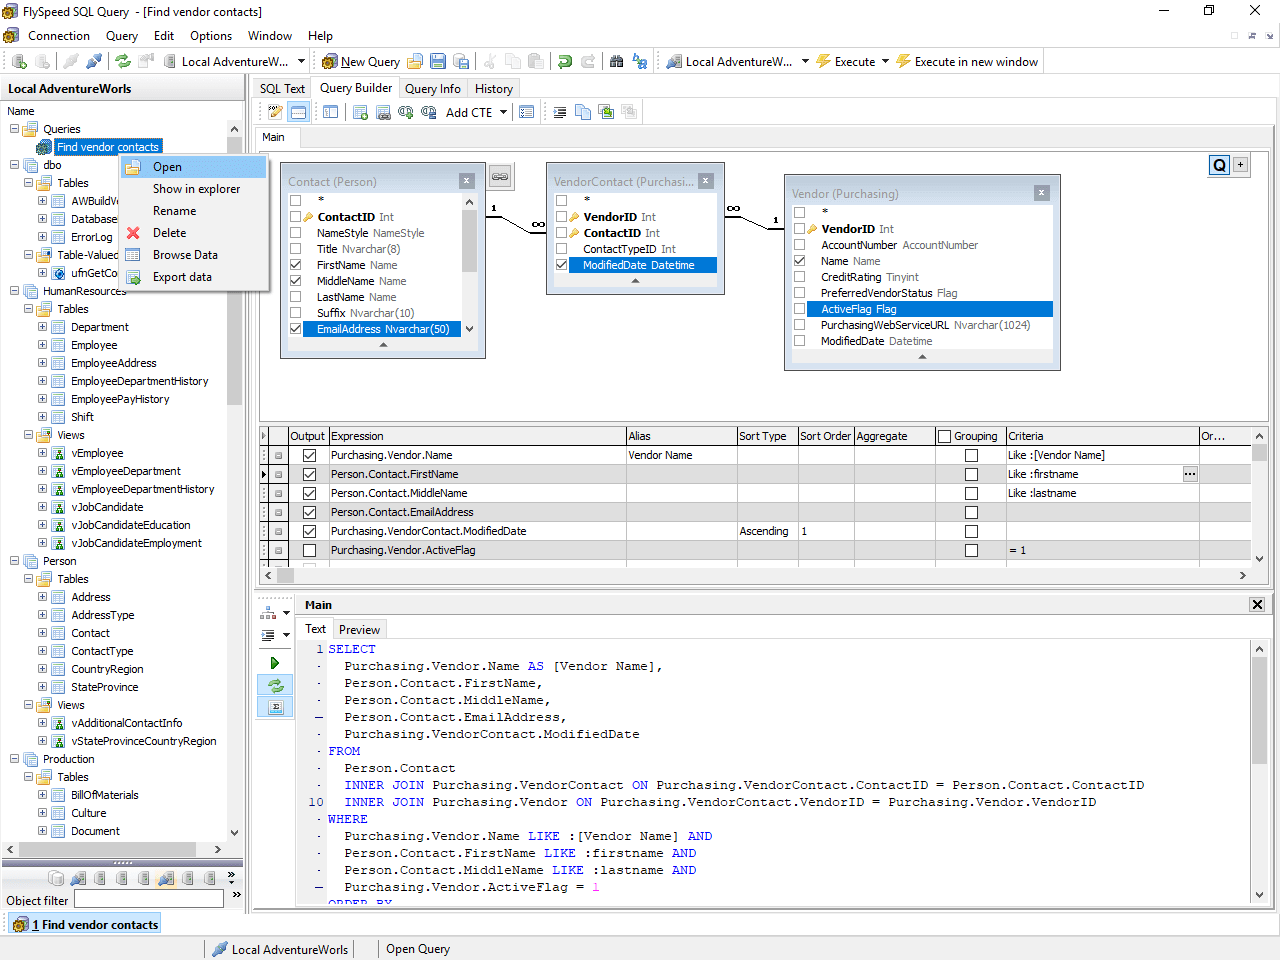
\includegraphics[width=1\textwidth]{img/flyspeed_1.png}
		\caption{Визуальное представление запроса в FlySpeed SQL Query}
		\label{analysis:flyspeed_1}}
\end{figure}  

\newpage

\subsection{Сравнение существующих решений}

На рисунке \ref{analysis:etl_compare} приведено сравнение существующих решений.

\begin{figure}[ht!]
	\centering{
		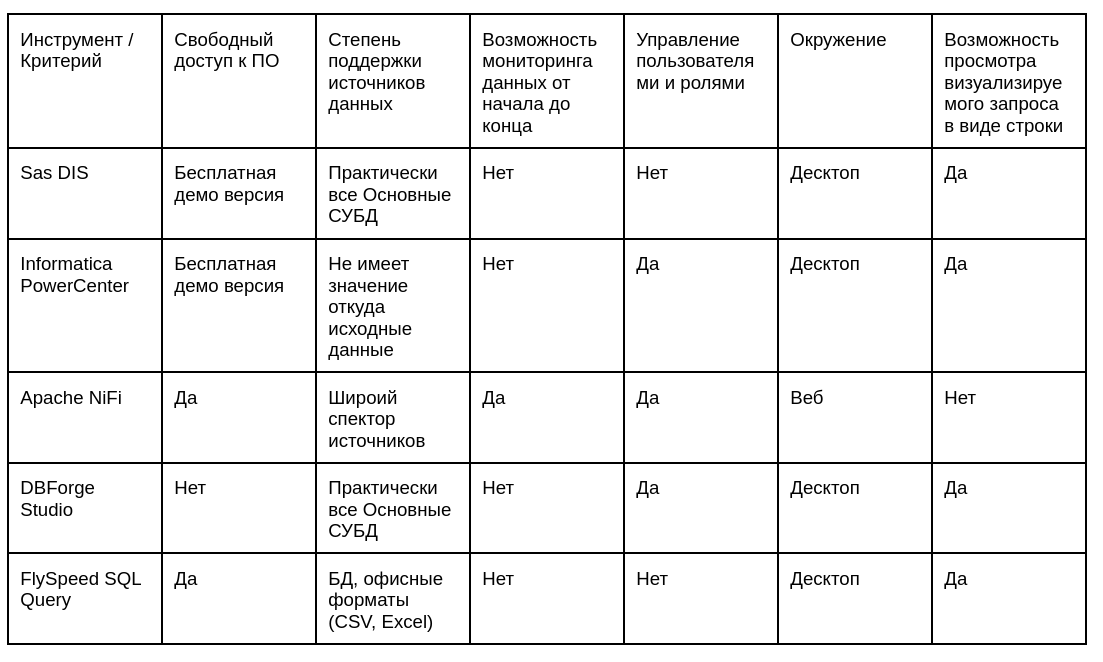
\includegraphics[width=1\textwidth]{img/etl_compare2.png}
		\caption{Сравнение существующих решений}
		\label{analysis:etl_compare}}
\end{figure}


\newpage

\section{План выполнения запроса PostgreSQL}

PostgreSQL получает на вход набор sql команд и обрабатывает каждую команду команду в четыре шага.

\begin{enumerate}
	\item Синтаксический анализ sql-запроса и последующее создание дерева синтаксического анализа.
	\item Оптимизация запроса.
	\item Создание плана.
	\item Выполнение.
\end{enumerate}

В PostgreSQL функция exec\_simple\_query выполняет представленные шаги.
Рассмотрим более подробно данные шаги.

\subsection{Построение дерева синтаксического анализа}

\textit{Дерево синтаксического анализа} -- набор хранимых в памяти взаимосвязанных типов. 
В случаи PostgreSQL этот набор хранимых структур данных языка Си \cite{bib1}.

С помощью синтаксического анализа PostgreSQL конвертирует sql-запрос во 
внутреннюю структуру данных, с которой в дальнейшем он может работать.

PostgreSQL использует генератор синтаксического анализа Bison \cite{bib5} для 
синтаксического анализа.

% Это легко ищется. перевормулировать.
Во время процесса сборки PostgreSQL Bison генерирует 
код парсера на основании ряда грамматических правил. 
Данный код работает внутри PostgreSQL, когда ему отправляются sql команды.
Далее каждое грамматическое правило вызывается, 
когда сгенерированный парсер находит соответствующий 
паттерн или синтаксис в строке sql и вставляет новую структуру памяти Си
в дерево синтаксического анализа \cite{bib12}.

Для примера рассмотрим следующий запрос 

\begin{lstlisting}[language=sql, label=some-code, caption=Пример sql-запроса над таблицей foo]
SELECT * FROM foo where bar = 42 ORDER BY id DESC LIMIT 23;
\end{lstlisting}

Данный запрос преобразуется в следующее дерево синтаксического анализа.

\begin{lstlisting}[language=sql, label=some-code, caption=Дерево синтаксического анализа для sql-запроса над таблицей foo]
(
   {SELECT 
   :distinctClause <> 
   :intoClause <> 
   :targetList (
      {RESTARGET 
      :name <> 
      :indirection <> 
      :val 
         {COLUMNREF 
         :fields (
            {A_STAR
            }
         )
         :location 7
         }
      :location 7
      }
   )
   :fromClause (
      {RANGEVAR 
      :schemaname <> 
      :relname foo 
      :inhOpt 2 
      :relpersistence p 
      :alias <> 
      :location 14
      }
   )
   :whereClause 
      {AEXPR  
      :name ("=")
      :lexpr 
         {COLUMNREF 
         :fields ("bar")
         :location 24
         }
      :rexpr 
         {A_CONST 
         :val 42 
         :location 30
         }
      :location 28
      }
   :groupClause <> 
   :havingClause <> 
   :windowClause <> 
   :valuesLists <> 
   :sortClause (
      {SORTBY 
      :node 
         {COLUMNREF 
         :fields ("id")
         :location 42
         }
      :sortby_dir 2 
      :sortby_nulls 0 
      :useOp <> 
      :location -1
      }
   )
   :limitOffset <> 
   :limitCount 
      {A_CONST 
      :val 23 
      :location 56
      }
   :lockingClause <> 
   :withClause <> 
   :op 0 
   :all false 
   :larg <> 
   :rarg <>
   }
)
\end{lstlisting}

Рассмотрим еще один запрос (листинг 1.3). 
На рисунке \ref{analysis:pg_step_1_tree} проиллюстрировано дерево синтаксического анализа, 
которое создал PostgreSQL из запроса представленного в листинге 1.3.

\begin{lstlisting}[language=sql, label=some-code, caption=Пример sql-запроса над таблицей users]
SELECT * FROM users
WHERE name = 'Captian Nemo'
ORDER BY id ASC
LIMIT 1;
\end{lstlisting}

\begin{figure}[ht!]
	\centering{
		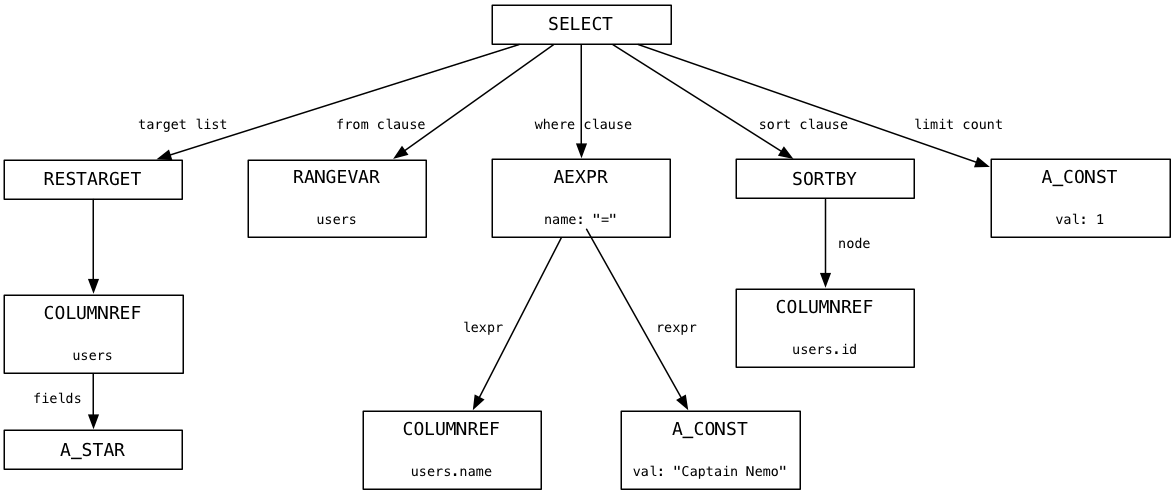
\includegraphics[width=1\textwidth]{img/pg_step_1_tree.png}
		\caption{Дерево синтаксического анализа для sql-запроса из таблицы users}
		\label{analysis:pg_step_1_tree}}
\end{figure}

\subsection{Оптимизация}

После того, как PostgreSQL создал дерево синтаксического анализа из переданного ему sql-запроса,
он преобразовывает его, применяя оптимизации, в другое дерево, используя другой набор узлов.
Полученное дерево называется деревом запроса.
Процесс оптимизации применяет ряд сложных алгоритмов и эвристик в 
попытке оптимизировать и упростить sql-запрос.

Для приведенного выше запроса (листинг 1.3) PostgreSQL преобразовал дерево 
синтаксического анализа в дерево,
представленное на рисунке \ref{analysis:pg_step_2_tree}.

\begin{figure}[ht!]
	\centering{
		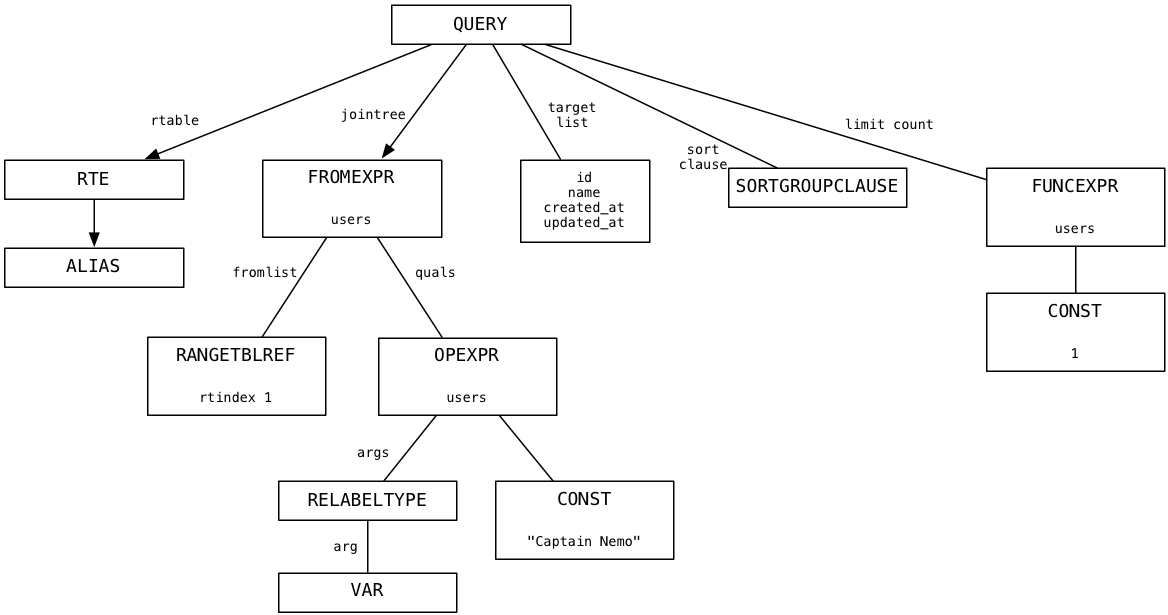
\includegraphics[width=1\textwidth]{img/pg_step_2_tree.png}
		\caption{Дерево запроса для sql-запроса из таблицы users}
		\label{analysis:pg_step_2_tree}}
\end{figure}

\subsection{Создание плана}

Перед тем, как начать выполнять запрос, PostgreSQL создает план.
Данный процесс включает в себя создание третьего дерева узлов, 
которые представляют собой список инструкций для PostgreSQL.
Для приведенного выше запроса (листинг 1.3) PostgreSQL построил 
дерево плана, которое показано на рисунке \ref{analysis:pg_step_3_tree}.

\begin{figure}[ht!]
	\centering{
		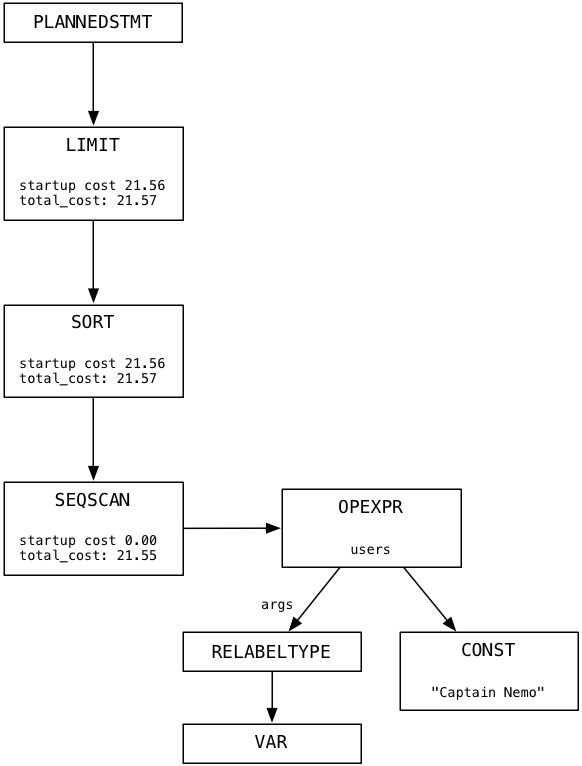
\includegraphics[width=0.6\textwidth]{img/pg_step_3_tree.png}
		\caption{План для sql-запроса из таблицы users}
		\label{analysis:pg_step_3_tree}}
\end{figure}

\newpage

\subsection{Выполнение}

На шаге выполнения запроса PostgreSQL уже преобразовал переданный ему в с самом начале 
sql-запрос в синтаксическое дерево анализа, оптимизировал и построил план запроса.
PostgreSQL имеет план, которому будет следовать, чтобы получить результат.
PostgreSQL для каждого нижележащего узла берет данные и возвращает их 
в качестве исходных данных для узла выше. 
Таким образом данный итеративный процесс повторяется,
пока что не будут получены данные из самого верхнего узла.
Это и будет являться результатом sql-запроса.

\section{Спецификация SQL запроса}

В данном разделе будет рассмотрена спецификация SQL запроса стандарта 602SQL.
Далее, описанные в данном разделе данные, потребуются для описания и реализации собственной грамматики.

\subsection{Спецификация query\_specification}

В основе SQL-select запроса лежит query\_specification.
Спецификация запроса выбирает набор выходных записей из записей из обобщенных таблиц. %  TODO: или создает
Если установлено предложение DISTINCT, будут выбраны только разные (уникальные) записи. %(только для столбцов фиксированной длины). 
Если ключевое слово ALL установлено (или опущено), будут выбраны все подходящие записи.
Если указано предложение WHERE, будут выбраны только те записи, которые удовлетворяют условию where\_condition.
Если указано предложение GROUP BY, записи будут разделены на группы. 
Каждая группа содержит записи с одинаковыми значениями выражения expression\_group.
Если указано предложение HAVING, будут выбраны только те группы, которые удовлетворяют условию having\_condition.
Если задано rename, то результирующая таблица будет переименована в name.
Выражение SELECT также может использовать символ '*',.
Если выражение имеет форму generalized\_table.*, все столбцы обобщенной таблицы будут в результате. 
Далее будут подробно рассмотрены элементы запроса.

\begin{lstlisting}[language=sql, label=some-code, caption=Спецификация SQL запроса]
   query_specification ::= SELECT [ ALL | DISTINCT ] expression [ rename ] { , expression [ rename ] } 
   FROM generalized table { , generalized table } 
   [ WHERE where_condition ] 
   [ GROUP BY expression_group { , expression_group } ]
   [ HAVING having_condition ]
   rename ::= AS name
\end{lstlisting}

\subsection{Спецификация query\_expression}

query\_expression  позволяет выполнять операции UNION, INTERSECT и EXCEPT над результатом  query\_specification
Операция UNION объединяет наборы записей, 
операция EXCEPT представляет различие, 
а операция INTERSECT показывает только сходство. 
Если ключевое слово ALL не указано, то каждая запись может быть в результате только один раз.

Если CORRESPONDING не установлен, предполагается, что оба операнда имеют одинаковое количество
столбцов и типы соответствующих столбцов одинаковы. Эти столбцы будут в результате.
Результат выражения запроса сортируется в соответствии со значениями выражения ORDER BY.
LIMIT задает количество записей в результате.

\begin{lstlisting}[language=sql, label=some-code, caption=Спецификация query\_expression]
   query_expression ::= { query_term | query_expression { UNION | EXCEPT } [ ALL ] 
   [ corresponding ] query_term } [ sorting ] [ selection ]
   query_term ::= query_specification  | query_term INTERSECT [ ALL ] [ corresponding ]  query_specification
   corresponding ::= CORRESPONDING [ BY ( column_name {, column_name } ... )]
   sorting ::= ORDER BY expression [ ASC | DESC ] {, expression [ASC | DESC ] } ... 
   selection ::= LIMIT [ offset , ] count
\end{lstlisting}

\subsection{Спецификация expression}

expression - это запись, состоящая из элементов, которую можно вычислить. 

\begin{lstlisting}[language=sql, label=some-code, caption=Спецификация SQL запроса]
   expression ::= simple_expression { operator simple_expression } ...
   simple_expression ::= literal          |
                     column_name          |
                     constants            |
                     subquery             |
                     CASE_expression      |
   operator ::=  + | - | * | / | MOD | DIV | chaining
\end{lstlisting}

Текст в языке SQL состоит из лексических элементов следующих типов.
\begin{enumerate}
   \item Зарезервированных слов.
   \item Идентификаторов - стандартные идентификаторы в языке SQL начинаются с буквы или подчеркивания ("\_") и могут содержать буквы, цифры и подчеркивания.
   \item Разделителей.
   \item Литералов.
   \item Комментариев.
\end{enumerate}

Литералы используются для ввода фиксированного значения в текст оператора SQL. 
Литералы бывают нескольких типов.

\begin{enumerate}
   \item number - представляет целое число, вещественное или полулогарифмическое.
   \item character\_string - представляет последовательность символов. Строки символов заключаются в апострофы при использовании в SQL. 
   Если строка символов содержит символ апострофа, его необходимо ввести дважды.
   \item binary\_string. Двоичные строки вводятся в шестнадцатеричном формате или в виде порядка байтов, заключенных в апострофы:
   % Символ X должен быть указан перед первым апострофом в шестнадцатеричной системе счисления, и каждый байт записывается как два шестнадцатеричных числа.
   % Символ B должен быть указан перед первым апострофом в байтовой записи, и каждый байт записывается как восемь цифр 0 или 1.
   \item date\_and\_time\_notation - обозначение времени и даты.  
\end{enumerate}

\begin{lstlisting}[language=sql, label=some-code, caption=Спецификация SQL запроса]
   literal ::= number | character_string | binary_string | date_and_time_notation
\end{lstlisting}

Имя столбца может быть (и должно быть, если может возникнуть дублирование столбцов) с префиксом имени таблицы или с псевдонимом таблицы.

\begin{lstlisting}[language=sql, label=some-code, caption=Спецификация SQL запроса]
   column_name ::= [table_name.]column_name
\end{lstlisting}

Подзапрос - вложенный запрос, содержащийся в предложении WHERE или HAVING другого оператора SQL.

\begin{lstlisting}[language=sql, label=some-code, caption=Спецификация SQL запроса]
   subquery ::= ( query_expression )
\end{lstlisting}

Выражение CASE служит для выбора значения одного из выражений на основе заданных условий. 
Ищется первая ветвь WHEN (слева направо), где значение expression2 совпадает со значением expression1 в данном CASE. 
Ищется первая ветвь WHEN (слева направо), где выполняется условие в условном CASE. 
Если подходящая ветвь найдена, значение выражения CASE будет expression3 в этой ветви. 
Если подходящая ветвь не найдена, значением выражения CASE будет expression4 или NULL, если expression4 не указано.
Все выражения expression2 должны иметь тип, сравнимый с expression1. 
Все выражения expression3 и expression4 должны быть преобразуемы в определенный общий тип.

\begin{lstlisting}[language=sql, label=some-code, caption=Спецификация SQL запроса]
   CASE_expression ::= simple_CASE | conditional_CASE
   simple_CASE ::= CASE expression1 { WHEN expression2 THEN expression3 } [ ELSE expression4 ] END
   conditional_CASE ::= CASE { WHEN condition THEN expression3 } [ ELSE expression4 ] END
\end{lstlisting}

\subsection{Спецификация generalized\_table}

Выражение join объединяет записи из двух таблиц путем связывания значений 
столбцов одной записи из первой таблицы и одной записи из второй таблицы. 
join\_type и join\_specification задают метод объединения записей из таблиц.

CROSS JOIN означает, что каждая запись соединяется со всеми записями из другой таблицы.
NATURAL означает, что две обобщенные таблицы должны иметь столбец с одинаковым именем. 
USING означает, что будут объединены только те записи, 
которые имеют одинаковые значения в указанных столбцах.
LEFT JOIN означает, что каждая запись из первой таблицы
должна быть соединена с некоторой записью (хотя бы одной) из второй таблицы. 
RIGHT JOIN означает, что каждая запись из второй таблицы
должна быть соединена с некоторой записью (хотя бы одной) из первой таблицы
FULL JOIN означает, что каждая запись из таблицы должна быть соединена
с записью (хотя бы одной) из противоположной таблицы.
INNER JOIN или JOIN означает, что записи, соответствующие join\_specification, должны быть объединены.

\begin{lstlisting}[language=sql, label=some-code, caption=Спецификация generalized\_table]
   generalized_table ::= { table_identifier [ index_specification ] 
    | stored_query_identifier | system_query | ( query_expression ) | join }
    [ rename ]
   index_specification ::= INDEX index_name
   join ::= generalized_table join_type generalized_table [ join_specification ]
   join_type ::= CROSS JOIN | [ NATURAL ] [ INNER | { LEFT | RIGHT | FULL } [ OUTER ] ] JOIN 
   join_specification ::= ON condition | USING ( column_name { , column_name } )
   rename ::= [ AS ] name [( column_name { , column_name } )]
\end{lstlisting}

\subsection{Спецификация condition}

condition - это выражение, которое может быть true, false или unknown.
condition используется для оценки оператора CASE, предложений WHERE и HAVING в спецификации запроса.
Приоритет оператора в condition определяется следующим образом:

\begin{itemize}
   \item *,/,DIV и MOD для умножения, деления, деления без остатка и модуля
   \item +, - для сложения и вычитания.
   \item Операторы отношения <,>,=,>=,<=,<>,.=,.=.,~ и предикаты (BETWEEN, LIKE и т. д.)
   \item НЕ оператор
   \item И оператор
   \item оператор ИЛИ
\end{itemize}

\begin{lstlisting}[language=sql, label=some-code, caption=Спецификация condition]
condition ::= boolean_factor { OR boolean_factor }
boolean_factor ::= boolean_expression { AND boolean_expression }
boolean_expression ::= [ NOT ] predicate
predicate ::= expression relational_operator expression    
      | IS_predicate 
      | generalized_comparison    
      | between_predicate   
      | in_predicate
      | EXISTS_predicate
      | UNIQUE_predicate
      | LIKE_predicate 
      | IS_NULL_predicate
      | Fulltext predicate
      | privilege_predicates
      | ( condition )
relational_operator ::= > | < | <= | >= | = | <>
IS_predicate ::= expression IS [NOT] { TRUE | FALSE | UNKNOWN }
\end{lstlisting}

% \subsubsection{Спецификация generalized\_comparison}
generalized\_comparison  сравнивает значение с набором значений из результата query\_expression (подзапроса).
Если quantifier является SOME или ANY, 
то обобщенное сравнение будет равно TRUE, если отношение 
допустимо хотя бы для одного из значений результата подзапроса.
Результатом будет unknown, если отношение unknown 
хотя бы для одного из значений результата подзапроса, в противном случае оно будет false.
Если quantifier равен ALL, то обобщенное сравнение будет равно true, 
если отношение для всех значений результата подзапроса допустимо. 

\begin{lstlisting}[language=sql, label=some-code, caption=Спецификация generalized\_comparison]
   generalized_comparison ::= expression  relational_operator quantifier ( query_expression )
   relational_operator ::= < | > | = | <= | >= | <> 
   quantifier  ::= SOME | ANY | ALL
\end{lstlisting}

Предикат BETWEEN указывает, находится ли expression между значениями expression2 и expression3. 
Типы все выражений должны быть совместимы.

\begin{lstlisting}[language=sql, label=some-code, caption=Спецификация between\_predicate]
   between_predicate ::= expression [ NOT ] BETWEEN expression2 AND expression3
\end{lstlisting}

in\_predicate указывает, находится ли значение expression1 среди значений указанных
expression или среди значений результата query\_expression (подзапроса).

\begin{lstlisting}[language=sql, label=some-code, caption=Спецификация in\_predicate]
   in_predicate ::= expression1 [NOT] IN {( expression { , expression } ) | ( query_expression )}
\end{lstlisting}

Предикат EXISTS определяет, есть ли хотя бы одна запись в результате подзапроса.

\begin{lstlisting}[language=sql, label=some-code, caption=Спецификация EXISTS\_predicate]
   EXISTS_predicate ::= EXISTS ( query_expression )
\end{lstlisting}

Предикат UNIQUE сообщает, все ли записи в результате query\_expression (подзапроса)
имеют уникальные значения. Учитываются только строки, не содержащие значение NULL.

\begin{lstlisting}[language=sql, label=some-code, caption=Спецификация UNIQUE\_predicate]
   UNIQUE_predicate ::= UNIQUE ( query_expression )
\end{lstlisting}

Предикат LIKE позволяет сравнить expression с expression2. 
Все выражения должны иметь тип character string.
Содержимое expression сравнивается с expression2 посимвольно со следующими исключениями: 
символ подчеркивания «\_» в expression2 соответствует любому одиночному символу в выражении, 
а символ процента «\%» в expression2 соответствует любой строке символов (даже пустой) в expression.

\begin{lstlisting}[language=sql, label=some-code, caption=Спецификация LIKE\_predicate]
   LIKE_predicate ::= expression [ NOT ] LIKE expression2 [ ESCAPE expression3 ]
\end{lstlisting}

IS\_NULL\_predicate позволяет сравнивать значение expression с null типом.

\begin{lstlisting}[language=sql, label=some-code, caption=Спецификация IS\_NULL\_predicate]
   IS_NULL_predicate::= expression IS [ NOT ] NULL
\end{lstlisting}

Fulltext predicate позволяет искать документы в fulltext system,
содержащие определенные слова, фразы или комбинации, 
используя операторы AND, OR, NOT и NEAR или используя круглые скобки.

privilege\_predicates представляет пять специальных предикатов для определения привилегий указанных
с учетом таблицы или записей таблицы. 
Этими предикатами являются has\_select\_privil(для привилегии чтения), 
has\_update\_privil (для привилегии обновления), 
has\_delete\_privil (для привилегии удаления), 
has\_insert\_privil (для привилегии вставки) 
и has\_grant\_privil (для привилегии предоставления).

\section{Формальные языки}

В данном разделе изложены некоторые аспекты теории формальных языков, существенные с точки зрения трансляции и построения дерева синтаксического анализа \cite{bib19}. 
В данном разделе будут введены базовые понятия и будут даны определения, связанные с одним из основных механизмов определения языков -- грамматиками, будет приведена
классификация грамматик по Хомскому \cite{bib20}.
Особое внимание уделяется контекстно-свободным и регулярным грамматикам \cite{bib21}. 
Грамматики этих классов используются при трансляции языков программирования. 

\subsection{Оснонвые понятия}

\textit{Алфавит} — это конечное множество символов.

\textit{Терминальные символы} - атомы, обозначим их строчными буквами ($a$, $b$, \dots).

\textit{Нетерминальные символы} -  это те символы, которые можно заменить, обозначим их заглавными буквами ($A$, $B$, \dots). 

\textit{Цепочкой символов} в алфавите $V$ называется любая конечная последовательность 
терминальных символов этого алфавита, обозначим графическими буквами ($\alpha$, $\beta$, \dots ) 

\textit{Цепочка}, которая не содержит ни одного символа, называется пустой цепочкой. 
Для ее обозначения будет использоваться греческая буква $\varepsilon$.

Обозначим через $V^{*}$ множество, содержащее все цепочки в алфавите
$V$, включая пустую цепочку $\varepsilon$.

Обозначим через $V{+}$ множество, содержащее все цепочки в алфавите $V$,
исключая пустую цепочку $\varepsilon$.

\textit{Язык в алфавите $V$} — это подмножество множества всех цепочек в этом алфавите. 
Для любого языка $L$ справедливо $L \subseteq V^{*}$.


\textit{Порождающая грамматика $G$} — это четверка $\left\langle {T, N, P, S} \right\rangle$, где
\begin{enumerate}
   \item T -- алфавит терминальных символов (терминалов);
   \item N -- алфавит нетерминальных символов (нетерминалов), $T \cap N = \varnothing$;  
   \item P -- конечное подмножество множества $(T \cup N)^{+} \times (T \cup N)^{*}$; 
   элемент $(\alpha, \beta)$ множества $P$ называется правилом вывода и записывается в виде $\alpha \rightarrow \beta$; 
   $\alpha$ -- называется левой частью правила, 
   $\beta$ -- правой частью; левая часть любого правила из $P$ обязана содержать хотя бы один нетерминал; 
\end{enumerate}

\textit{Языком}, порождаемым грамматикой $G = \left\langle {T, N, P, S} \right\rangle$, 
называется множество $L(G) = \{ \alpha \in T^{*} | S \Rightarrow \alpha \}$ 

\subsection{Классификация грамматик и языков по Хомскому}

По Иерархии Хомского, классификация формальных языков 
и формальных грамматик делится на следующие 4 типа.

\begin{enumerate}
   \item Неограниченные (Тип 0).
   \item Контекстно-зависимые (Тип 1).
   \item Контекстно-свободные (Тип 2).
   \item Регулярные (Тип 3). 
\end{enumerate}

\subsubsection{Неограниченные}

Любая порождающая грамматика является грамматикой типа 0. 
На вид правил грамматик этого типа не накладывается никаких дополнительных ограничений. 
Класс языков типа 0 совпадает с классом рекурсивно перечислимых языков. 

\subsubsection{Контекстно-зависимые}

Грамматика $G = \left\langle {T, N, P, S} \right\rangle$ называется контекстно-зависимой (КЗ),
если каждое правило из $P$ имеет вид $\alpha \rightarrow \beta$, где $\alpha = \xi_1A\xi_2$, 
$\beta = \xi_1 \gamma \xi_2$, $A \in N$, $\gamma \in (T \cup N)^{+}$, $\xi_1, \xi_2 \in (T \cup N)^{*}$

В виде исключения в КЗ-грамматике допускается наличие правила с пустой правой частью
$S → \varepsilon$, при условии, что $S$ (начальный символ) не встречается в правых частях правил.

Цепочку $\xi_1$ называют левым контекстом, цепочку $\xi_2$ называют правым контекстом. 
Язык, порождаемый контекстно-зависимой грамматикой, называется контекстнозависимым языком.

\subsubsection{Контекстно-свободные}

Грамматика $G = \left\langle {T, N, P, S} \right\rangle$ называется контекстно-свободной (КС),
если каждое правило из $P$ имеет вид $A \rightarrow \beta$, где $A \in N$,
$\beta \in (T \cup N)^{*}$

Впервые КС-грамматики были использованы для описания синтаксиса алгоритмических 
языков в \cite{bib22}. Формализм металингвистических формул, названный позднее BNF-формой, 
в \cite{bib23} был дополнен возможностью использовать регулярные выражения над терминалами, 
нетерминалами в правых частях правил и получил еще одну букву в обозначении класса грамматик RBNF. 

\subsubsection{Регулярные}

Грамматика $G = \left\langle {T, N, P, S} \right\rangle$ называется \textit{праволинейной},
если каждое правило из $P$ имеет вид $A \rightarrow wB$, либо $A \rightarrow w$, 
где $A, B \in N$, $w \in T^{*}$ 

Грамматика $G = \left\langle {T, N, P, S} \right\rangle$ называется \textit{леволинейной},
если каждое правило из $P$ имеет вид $A \rightarrow Bw$, либо $A \rightarrow w$, 
где $A, B \in N$, $w \in T^{*}$ 

Праволинейные и леволинейные грамматики определяют один и тот же класс языков. 
Такие языки называются регулярными. 
Праволинейные и леволинейные грамматики называются регулярными.

% На рисунке показан процесс преобразования исходной программы в asm команды.
% \begin{figure}[ht!]
% 	\centering{
% 		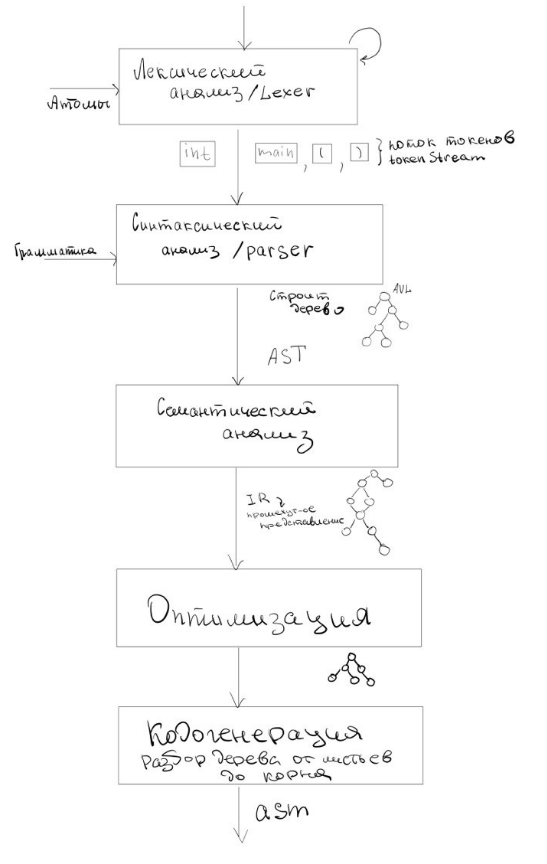
\includegraphics[width=0.6\textwidth]{img/compilation_process.png}
% 		\caption{Процесс преобразования исходной программы в asm команды}
% 		\label{analysis:compilation_process}}
% \end{figure}


% \section{Грамматика}


